% Compile with: pdflatex (run twice for the table of contents)
\documentclass[12pt,a4paper]{article}

\usepackage[margin=2.5cm]{geometry}
\usepackage{booktabs}
\usepackage{array}
\usepackage{graphicx}
\usepackage{amsmath}
\usepackage[hidelinks]{hyperref}
\usepackage{caption}
\usepackage{float}
\usepackage{tikz}
\usetikzlibrary{arrows.meta,positioning,fit,backgrounds,calc,shapes.geometric}
% Long unbreakable tokens (citation keys, slash lists, URLs) otherwise force
% minor overfull boxes; let TeX stretch interword space in the final pass.
\setlength{\emergencystretch}{2.5em}

% LaTeX's defaults (topnumber=2, totalnumber=3) spread 14 floats across many
% pages, so a float can land ten pages after the sentence that cites it.
% Relaxing them keeps each float within a page or two of its reference.
\setcounter{topnumber}{4}
\setcounter{bottomnumber}{3}
\setcounter{totalnumber}{6}
\renewcommand{\topfraction}{0.85}
\renewcommand{\bottomfraction}{0.7}
\renewcommand{\textfraction}{0.08}
\renewcommand{\floatpagefraction}{0.75}
% Never let a float drift past the end of its own section.
\usepackage[section]{placeins}
\hyphenation{odometry teleoperation downstream}
\captionsetup{font=small,labelsep=quad}

% Ragged-right column type for tables that hold running prose.
% Justified narrow columns stretch interword space and break words like
% "mech-anism" and "coopera-tion" across lines, which is much harder to read
% than a slightly ragged right edge.
\newcolumntype{L}[1]{>{\raggedright\arraybackslash}p{#1}}
\newcolumntype{R}{>{\raggedleft\arraybackslash}p{1.4cm}}

% Shared TikZ styles for the diagrams.
\tikzset{
  block/.style   = {draw, rounded corners=2pt, align=center, inner sep=4pt,
                    minimum height=8mm, font=\footnotesize, fill=white},
  copyblk/.style = {block, fill=blue!8},
  predblk/.style = {block, fill=orange!12},
  resblk/.style  = {block, fill=red!8},
  ioblk/.style   = {block, fill=black!5},
  flow/.style    = {-{Latex[length=1.6mm]}, semithick},
  copflow/.style = {flow, dashed, blue!55!black},
}

\title{Residual-Triggered Data Acquisition: From Cerebellum-Style Sensory Prediction to a Data-Acquisition Protocol Layer\\[4pt]
\large --- A Perspective with Prototype Validation}
\author{}
\date{September 2026}

\begin{document}

\maketitle

\begin{abstract}
Cameras are shifting from ``on demand'' to ``always on'': robot arms, AR glasses and home robots each generate hundreds of gigabytes of raw video per day, of which only a few percent is ever used. Paying the full storage, bandwidth and annotation cost to recover single-digit-percent value is the central data-collection problem of always-on sensing. We pursue one route, \textbf{residual-triggered data acquisition}, which borrows the three-element architecture of cerebellum-like circuits: instead of detecting \emph{what is important}, the device predicts \emph{what change it caused itself} and stores only the unpredicted residual.

\textbf{Positioning.} The layer is a partial substitute, not a replacement, and it is not an alternative to optical flow. It displaces exactly one module---the cheap change detector that gates a keep-or-discard decision at capture---and only under five preconditions: a binary rather than field-valued decision, a frame-synchronised gyroscope, rotation-dominated motion, acceptable per-device calibration, and near-zero compute. If any fails, the layer is out of scope, and \textbf{dense optical flow is the better and more portable choice}: flow needs no IMU, calibration or vendor cooperation, degrades gracefully onto translation and parallax, improves with better models, and yields a field other components reuse. What this layer offers in exchange for those restrictions is cost---0.03--0.07\,ms/frame against 3.8--8.5\,ms/frame for flow.

\textbf{Results.} On a synthetic rig, storing 3.4\% of frames trains a downstream model better than uniform sampling at four times the budget and better than a full-budget oracle. On real egocentric video the advantage does not transfer: the trigger selects kinematically unpredictable frames rather than semantically important ones. Six negative results bound the layer to motion deduplication and bandwidth pre-filtering, and an ablation shows the sharpest real-data failure is not irreducible---it is the omission of roll from a two-axis predictor, correctable for 0.04\,ms/frame.

All numbers reported are measured values from a reproducible open-source prototype, and negative results are given the same weight as positive ones.
\end{abstract}

\noindent\textbf{Keywords:} residual-triggered data acquisition; corollary discharge; negative image; cerebellum-like circuits; sensory prediction; data filtering layer; IMU; event detection

\tableofcontents
\newpage

\section{Introduction: The Storage--Value Asymmetry of Always-On Cameras}

This is a perspective article with prototype validation rather than a systematic review. It argues for an architectural position and then holds that position to a measured account rather than surveying a literature, and it reports negative results with the same care as positive ones because they are what fix the method's applicability boundary. Coverage of adjacent literatures is deliberately selective---sufficient to locate the contribution, not exhaustive.

\subsection{The problem}

Cameras are shifting from ``on demand'' to ``always on.'' Three concrete scenarios illustrate the scale of the problem:

\begin{itemize}
  \item \textbf{Robot grasping}: a camera running at 30 fps produces about 270 GB of raw video per day. When an engineer reviews the footage a month later, they typically want only the few dozen failed-grasp clips---usually less than 3\% of the data.
  \item \textbf{AR glasses}: a month of continuous recording is roughly 8 TB, and 97\% of it is meaningless corridors and ceilings; uploading everything is unacceptable for privacy.
  \item \textbf{Embodied-data collection}: first-person manipulation datasets such as Open-AoE~\cite{openaoe} require thousands of hours of video followed by manual annotation, with annotation cost proportional to video duration---yet what is truly rare are failures, surprises, and long-tail actions.
\end{itemize}

The common structure: \textbf{storage costs scale linearly; value does not.} What is missing from the data path is a \textbf{filtering layer} that keeps only the few percent worth storing. This layer has three hard constraints:

\begin{enumerate}
  \item \textbf{Extremely cheap}---cheap enough to run always-on. A filter that spends 10\% of the energy budget on itself is unqualified: the storage it saves may not afford its own power bill.
  \item \textbf{Online and adaptive}---illumination, scene, and wearer behaviour all change; fixed thresholds trained offline are not acceptable.
  \item \textbf{Self-labelling}---the importance signal itself must not depend on human annotation or another expensive model.
\end{enumerate}

\subsection{Why existing routes are not enough}

\begin{table}[htbp]
  \centering
  \small
  \caption{Existing data-collection routes and their failure modes.}
  \label{tab:routes}
  \begin{tabular}{L{3.4cm}L{3.2cm}L{7.0cm}}
    \toprule
    Route & Idea & Failure mode \\
    \midrule
    Store/upload everything & Save first, filter later & Storage/bandwidth grow linearly with data volume; privacy-unacceptable \\
    Motion triggering (frame diff./PIR) & Record when the image changes & \textbf{The device's own} walking, turning, and hand shake are all ``change''---any change detection that ignores self-motion drowns (measured: frame differencing recalls 0 events under rotation) \\
    Specialised sensors (event cameras) & The sensor itself outputs only change & Requires new hardware; cost, dynamic range, and supply chain are unsuitable for existing consumer devices \\
    Learned importance scoring & Train a small model as judge & The judge itself needs expensive always-on perception, plus data maintenance \\
    Uniform/adaptive frame sampling & Sample within budget & A 5\% budget recalls only 17\% of events (measured) \\
    \bottomrule
  \end{tabular}
\end{table}

The technical crux of Table~\ref{tab:routes} is the second row: \textbf{within the signal ``the image changed,'' the largest, most frequent, and---crucially---most predictable component is the optic flow caused by the device's own motion.} Any change detection that does not handle self-motion is overwhelmed by it. This is precisely why frame differencing works for fixed surveillance and fails catastrophically on mobile devices.

\subsection{The core idea of this article, and its organization}

Invert the problem. Detecting ``what is important'' is hard (it amounts to doing semantic understanding on the device); but predicting ``what change I caused myself'' is easy---\textbf{because the device carries its own motion sensor (an IMU)}. The route is therefore:

\begin{enumerate}
  \item \textbf{Copy}: read the gyroscope and know how the camera is currently rotating;
  \item \textbf{Predict}: maintain per-cell running statistics on a deep feature map, learning ``how much change my own motion typically causes'';
  \item \textbf{Residual}: subtract the predicted component, and \textbf{trigger storage only where the residual is large}---what gets stored is the footage the device could not predict.
\end{enumerate}

The structure is borrowed from neuroscience---African weakly electric fish use a homologous circuit to subtract self-interference from prey signals---but its key advantage is engineering-side: \textbf{the IMU ships with every consumer device.} What event cameras need dedicated silicon for becomes a pure software problem here: zero training, zero annotation, about 0.2 ms per frame.

\subsection{What this replaces, and what it explicitly does not}
\label{sec:scope-intro}

It is easy to read ``a pluggable acquisition layer'' as a claim to replace perception front-ends in general. It is not. The claim is much narrower, and stating it precisely is what makes the contribution actionable.

The layer displaces \textbf{one module}: the cheap change detector that gates a capture decision---frame differencing, a background model, a motion-energy threshold, or an IMU-gated sampler. That is the only slot it fills. In the terms of Section~\ref{sec:related}, it is an acquisition-time \emph{selector}, and its output is a single scalar per frame whose only consumer is a keep-or-discard decision.

\begin{table}[htbp]
  \centering
  \small
  \caption{What the layer substitutes for, and what it does not. The distinction is the output type: a scalar gating decision versus a dense motion field. Only the former is in scope, which is why the two columns are complements rather than alternatives.}
  \label{tab:scope}
  \begin{tabular}{L{2.6cm}L{5.4cm}L{5.4cm}}
    \toprule
    & Residual triggering (this work) & Dense optical flow \\
    \midrule
    Output & one scalar per frame (novelty) & per-pixel motion field $(H{\times}W{\times}2)$ \\
    Sensor requirement & IMU, frame-synchronised & none \\
    Calibration & focal length $f_{\mathrm{map}}$ and per-axis signs per device/segment & none \\
    Vendor cooperation & needs the gyro stream exposed & none \\
    Open-set behaviour & rotation only; translation and parallax unmodellable & degrades gracefully to translation and parallax \\
    Upgrade path & better copy (more axes, better sync) & better learned model \\
    Cost & 0.03--0.07 ms/frame & 3.8--8.5 ms/frame \\
    Downstream reusability & none: the scalar is consumed by the trigger & high: EIS, frame interpolation, SLAM, depth \\
    \bottomrule
  \end{tabular}
\end{table}

Three consequences follow, and they are the reason the positioning matters more than the benchmark numbers.

\textbf{It cannot replace optical flow, and it does not compete with it on flow's terms.} Flow produces a dense motion field; this layer produces a scalar. A system that needs the motion field---for stabilisation, interpolation, structure from motion, or depth---cannot use this layer at all, and should not try. Conversely, a system that only needs to decide whether to keep a frame is paying for a motion field it will never read. The honest summary is that this layer trades almost everything flow offers in exchange for two orders of magnitude of cost, and that trade is only rational at one specific point in the stack: the always-on gate.

\textbf{Flow is the more compatible and more portable choice whenever it is affordable.} Flow needs no IMU, no calibration, no vendor licence, and no assumption about what kind of motion dominates; it is a drop-in for any camera, and it improves with every advance in the flow literature. This layer needs all four of those preconditions and its accuracy is capped by how well a rotation-only model describes the scene. Where the budget exists---offline or cloud processing, a robot with a GPU, a task requiring the motion field---\textbf{optical flow remains the better choice}, and the measured cost-quality picture of Section~\ref{sec:design} should be read as the price of not paying for it, not as a victory over it. The correct relationship is the arbitration cascade of Section~\ref{sec:arbiter}: this layer always-on and cheap, flow invoked on the candidates this layer proposes, so that flow's expense is confined to the small fraction of frames that survive the gate.

\textbf{Where it does land, it lands in a specific and useful place.} The realistic deployments are those where a coarse keep-or-discard decision at capture time is worth more than a precise motion estimate later, and where the device already carries a gyroscope. Three concrete cases: (i)~\emph{phone-based egocentric data collection}, where annotation cost scales with delivered duration and a 10\% capture rate is a 10$\times$ saving on the annotation budget, and where the OS already exposes the IMU to any app; (ii)~\emph{bandwidth-limited teleoperation or field robotics}, where the link cannot carry the full stream and the question is which clips to spend it on; (iii)~\emph{always-on consumer devices, and AR glasses in particular}, where privacy makes uploading everything unacceptable and an on-device gate that never leaves the device is the only compliant option. In all three, the layer is a pre-filter that runs upstream of---and never instead of---whatever the vision model does with the frames that survive.

The boundary is stated once more in Section~\ref{sec:scope} in the form of an explicit substitution test, so that a reader can decide in one step whether their setting is in scope.

The rest of this article is organized as a ``0 to 1'' narrative: Section~\ref{sec:bio} covers the biological origin; Section~\ref{sec:lineage} the intellectual lineage; Section~\ref{sec:eng} surveys homologous engineering structures and positions the idea against the neighbouring selection paradigms (Section~\ref{sec:related}); Section~\ref{sec:design} presents the prototype design and cost accounting; Section~\ref{sec:experiments} reports the experimental record, positive and negative; Section~\ref{sec:principles} distils transferable design principles; Section~\ref{sec:discussion} discusses boundaries and outlook.

\section{The Biological Origin: Corollary Discharge and the Negative Image}
\label{sec:bio}

\subsection{The problem: interfering with yourself}

Sensory systems universally face a problem: the animal's own actions contaminate its own sensations. The weakly electric fish \emph{Apteronotus leptorhynchus} is an extreme instance: it uses its electric organ discharge (EOD) for active sensing, generating a weak electric field and detecting deformations caused by prey. But its own EOD is several orders of magnitude stronger than prey signals at the receptors---\textbf{the fish drowns out the very target it wants to detect}.

The fish's solution is not a better detector but a three-element circuit~\cite{bell1981,bastian1986}:

\begin{enumerate}
  \item \textbf{Corollary discharge}: a copy of the motor command (the EOD command), expanded into a multi-timescale signal by granule cells and delivered to the electrosensory lateral line lobe (ELL);
  \item \textbf{Negative image}: MG cells in the ELL (functionally analogous to cerebellar Purkinje cells) use local plasticity to learn a precise prediction of self-interference---``given that I am discharging now, what will the receptors see?'';
  \item \textbf{Residual}: output cells (analogous to cerebellar deep nuclei) subtract the negative image and report only the unpredicted residual---the prey signal is \emph{subtracted out}, not \emph{detected}.
\end{enumerate}

\subsection{Connectomic evidence: this is a circuit, not a metaphor}

For decades this functional framework rested on inferences from electrophysiology and behaviour. Perks et al.\ (2026)~\cite{perks2026} provided the ultimate constraint: an electron-microscopy connectomic reconstruction of the entire microcircuit (29{,}694 synapses covering 88 output cells and 136 MG cells), directly testing whether the real synaptic wiring satisfies the theoretical requirements of the function. Three major findings:

\begin{enumerate}
  \item \textbf{Sensory input reaches the plastic cells via inhibitory and disinhibitory pathways.} Intuitively, electroreceptor afferents should excite MG cells directly; instead, the dominant pathway runs through two stages of interneurons: ON/MG$+$ cells receive two-stage inhibition (sign-preserving), OFF/MG$-$ cells receive one-stage inhibition (sign-inverting)---the teaching signal for plasticity requires a specific biophysical form, and the real wiring matches the design requirement exactly.
  \item \textbf{MG$\to$output-cell connectivity precisely solves credit assignment.} MG$-$ cells connect only to ON and MG$+$ cells; MG$+$ cells connect only to OFF and MG$+$ cells---only 1 of 3{,}527 MG$\to$output synapses violates the pattern, and MG--MG recurrent wiring is equally precise (10 violations among 1{,}322 synapses). The negative image is learned in MG cells and passed to the output cells.
  \item \textbf{Two plasticity sites plus recurrent connectivity $=$ fast, accurate, noise-robust.} A computational model constrained by the connectome reproduces in-vivo recordings; ablations show that with output-cell plasticity alone, OFF cells learn very slowly (potentiation is about $8\times$ slower than depression), while MG input lends the fast-learned half of the negative image to the slow half; adding MG recurrence makes both sides fast. The most important unit test is \textbf{noise robustness}: under continuous zero-mean exogenous noise injection, cancellation accuracy barely degrades---and this robustness depends critically on the \emph{coexistence} of both plasticity sites; removing either one collapses it.
\end{enumerate}

The engineering significance of these findings: \emph{predict-and-cancel} is not an optional biological detail but the generic solution of sensory systems under energy constraints. Evolution has independently arrived at the same architecture wherever a modality interferes with itself: the electrosense of electric fish, saccadic suppression in mammals, vocalization-induced suppression in bat echolocation and human hearing. When a device faces the homologous problem (self-motion contaminating vision), copying this architecture is a low-risk choice---provided each borrowed element is experimentally verified to still hold in engineering, which is exactly the content of Section~\ref{sec:experiments}.

\section{The Intellectual Lineage: Perception $=$ Prediction $+$ Residual}
\label{sec:lineage}

The idea of residual-triggered acquisition has a clear cross-disciplinary lineage:

\begin{itemize}
  \item \textbf{Helmholtz (1867)}: perception is ``unconscious inference''---sensory signals alone are insufficient, and the brain must combine them with priors.
  \item \textbf{von Holst \& Mittelstaedt (1950)}~\cite{vonholst1950}: distinguish \emph{reafference} (sensations caused by one's own actions) from \emph{exafference} (sensations caused by the environment), and propose that the nervous system holds a \textbf{copy of the motor command} to tell them apart---the origin of the corollary-discharge concept, explaining why the world appears stable during saccades.
  \item \textbf{The Marr--Albus--Ito cerebellar learning theories (1970s)}~\cite{marr1969,albus1971,ito1982}: the cerebellum as a supervised learning machine, with climbing fibres carrying error signals to modify parallel-fibre--Purkinje-cell synapses---the first theoretical formulation of error-driven learning via local plasticity.
  \item \textbf{Kawato / Wolpert (1980s--90s)}~\cite{kawato1992,wolpert2000}: the cerebellum hosts \textbf{internal forward models}---given the current state and a motor command, predict the sensory consequence; motor control, sensory attenuation (why self-tickling does not tickle), and saccadic suppression receive a unified explanation.
  \item \textbf{Rao \& Ballard (1999)}~\cite{raoballard1999}: predictive coding---residual response patterns in visual cortex are consistent with hierarchical inference of ``top-down prediction + bottom-up error.''
  \item \textbf{Bell \& Bastian (1990s--2000s)}~\cite{bell1981,bastian1986}: the ELL negative image of electric fish provides the cleanest electrophysiologically testable instance of the above ideas.
  \item \textbf{Perks et al.\ (2026)}~\cite{perks2026}: connectomics provides the ultimate constraint---this computation is a circuit of real synaptic connections, not a theorist's metaphor.
\end{itemize}

This lineage supports a single architectural judgement: \textbf{predict-and-cancel is the generic design pattern of sensory systems.} Prediction is autoregressive---you know what you just did; detection is open-set---you do not know what the world will produce. Given a copy of the motor command, predicting self-interference is several orders of magnitude easier than detecting external targets, so evolution (and good engineering) should spend the entire budget on the easy half and simply not do the hard half, or defer it.

\subsection{Why the asymmetry is structural, not incidental}

The claim that prediction is cheaper than detection is worth stating precisely, because the entire architecture rests on it and it is easy to mistake for a heuristic. The asymmetry is not about difficulty in the abstract; it is about \emph{the shape of the function class each side must represent}.

A predictor conditioned on a copy of the motor command solves a \emph{forward} problem: given an input $u_t$ that the system itself emitted, produce the sensory consequence. For rotation-induced optic flow this map is well-posed, low-dimensional (three angular rates to two image displacements), and---critically---\emph{independent of scene content beyond depth}. Equation~(1) contains no term that depends on what the camera is looking at. A world-motion detector solves the \emph{inverse} problem: given only the image, decide which of the observed changes were caused by the environment. That map is ill-posed, since infinitely many scene-plus-motion configurations produce the same image pair, and its dimensionality is the dimensionality of the world.

\begin{table}[htbp]
  \centering
  \small
  \caption{The structural asymmetry between the two halves of the sensory problem. The rows are properties of the \emph{function class}, not of any particular implementation, which is why the conclusion survives changes of backbone, feature map or trigger rule.}
  \label{tab:asym}
  \begin{tabular}{L{2.4cm}L{4.4cm}L{5.4cm}}
    \toprule
    Property & Predict self-change & Detect world-change \\
    \midrule
    Direction & forward (cause $\to$ effect) & inverse (effect $\to$ cause) \\
    Conditioning input & motor command $u_t$, known exactly & image only; cause latent \\
    Well-posedness & well-posed & ill-posed (many causes, one image) \\
    Dimensionality & 3 angular rates $\to$ 2 displacements & open-set: the world \\
    Scene dependence & none beyond depth & everything \\
    Cost scaling & $O(\text{pixels})$, content-independent & $O(\text{pixels}\times\text{search})$, content-dependent \\
    Failure when wrong & residual merely larger & silently misses the target \\
    \bottomrule
  \end{tabular}
\end{table}

Table~\ref{tab:asym} makes the strategic point explicit: the two halves differ not in how hard they are to \emph{approximate} but in whether a correct answer is even well defined. A method that is wrong about self-motion does not fail gracefully---it fails by \emph{having no residual to look at}, which is exactly the measured collapse of frame differencing under rotation (recall 0). This is the sense in which the protein is spent wisely: evolution cannot afford to solve the ill-posed half on every modality, so it solves the well-posed half exactly and lets the residual carry the rest.

There is a second, quieter argument from energy. A forward model can be evaluated \emph{before} the sensory event it predicts, since its input is the motor command. That means cancellation hardware can be prepared in advance and, in the limit, subtracted at the sensor---which is what the electrosensory system does and what event-camera silicon does in a different way. An inverse solver has no such option: it can only run after the fact, on data that must already have been captured and buffered. For an always-on device the difference is between a filter that can be upstream of storage and one that is necessarily downstream of it. This project is a software approximation to the upstream position, achieved cheaply by making the copy a sensor reading rather than a computation.

Finally, the lineage clarifies what is \emph{new} here. Von Holst's reafference principle, the Marr--Albus--Ito framework, internal forward models and predictive coding all agree that the brain predicts and subtracts; none of them addresses the engineering question of where such a filter belongs in a data path, or what happens when the predictor's function class is chosen badly. That is the gap the experimental record below fills, and it is why the negative results occupy as much space as the positive ones.

\section{Homologous Structures in Engineering}
\label{sec:eng}

Interestingly, predict-and-cancel is not new in computer science either; it is scattered across fields and rarely treated as a general principle:

\begin{itemize}
  \item \textbf{Video coding}: H.264/AVC P-frames do not transmit the full picture, only the motion-compensated residual~\cite{h264}. Prediction is easy on the encoder side (block matching against a known reference frame), so the transmission budget is spent entirely on what prediction misses. Residual-triggered storage moves this same structure from ``compress one video'' to ``filter one unbounded stream'': the predictor is replaced by an IMU copy (cheaper, texture-independent), and the residual's purpose changes from ``reconstruction'' to ``decide whether to store.''
  \item \textbf{Background modelling}: background subtraction~\cite{piccardi2004,bouwmans2014} is essentially ``learn the scene's negative image, report only the foreground residual.'' Its failure mode is fully homologous---as soon as the camera rotates, the background model is torn apart by self-motion. Two decades of improvement (e.g.\ PTZ camera angle readback) are essentially retrofitting the missing \emph{copy}, confirming from another angle that negative-image learning without a copy does not go far on mobile platforms.
  \item \textbf{Acoustic echo cancellation (AEC)}~\cite{benesty2001}: in teleconferencing, the loudspeaker leaks into the microphone. The naive solution---``hear the echo in the recording and subtract it''---is an open-set problem and extremely hard; deployed systems instead take \textbf{the loudspeaker playback signal as a reference copy} and use an adaptive filter to predict its room-transformed form at the microphone, then subtract.
  \item \textbf{Active noise-cancelling headphones}: the music signal itself serves as the reference to predict residual noise, rather than ``listening again.''
  \item \textbf{Model-based anomaly detection}: residual tests (build a baseline, flag outliers) are the mainstream paradigm of industrial anomaly detection. The residual trigger score is a $z$-scored residual---not a learned importance model.
  \item \textbf{Event cameras}: output only brightness changes at the silicon level~\cite{gallego2020}. Convergent with residual triggering (both answer ``transmit only change''), but they require dedicated hardware and discard the RGB context outside the residual---and context has downstream training value (in the synthetic benchmark of Section~\ref{sec:experiments} the residual-triggered clips even beat the full-budget oracle on event recall, partly because they preserve context).
\end{itemize}

\subsection{The copy is already in the stack---and only one platform exposes it}
\label{sec:stack}

The corollary discharge is not exotic hardware. Every serious camera pipeline already consumes the gyroscope: gimbals use it \emph{in closed loop} (feedback control), electronic stabilization uses it \emph{in post-processing} (alignment warps between frames), and rolling-shutter correction uses it \emph{in modelling} (per-row exposure time $\times$ angular rate). This project adds a fourth consumer: \emph{prediction}---using the same signal to know what the next frame should look like, and hence which part of it is not worth storing. The four uses share one premise: the cause of image change is a known variable rather than an unknown to be estimated.

This is also the precise answer to ``what is different about video-plus-gyro data?'' Plain video shows only effects; self-motion must be estimated from the image itself---an inverse problem that is ill-posed, texture-dependent, and costs 3.8 ms/frame with dense optical flow. With the gyro, the cause is a measured input, and prediction becomes a well-posed forward problem: an $O(\text{pixels})$ shift costing 0.03 ms. Self-motion changes from noise to be suppressed into a known quantity to be subtracted---which is why the residual that remains reports on the world instead of the device.

Platform accessibility then decides where such a layer can live. Action-camera vendors (GoPro, Insta360, DJI) treat the raw gyro stream as core IP---it is literally the product (HyperSmooth, FlowState, three-axis stabilization)---and expose it only under SDK agreements and NDAs. On phones, the gyroscope is served by standard OS sensor APIs (Android SensorManager, iOS CoreMotion) at 100+ Hz with hardware timestamps, with no vendor licence and no user permission prompt; a generic logging app suffices. Phones are the only mass-market platform whose sensor data plane is open while the camera module is good enough. Crucially, this is not a compromise: the acquisition scenarios the layer targets are dominated by phone footage (Open-AoE~\cite{openaoe} is entirely phone-captured), so the platform where the copy is obtainable coincides with the platform where the data is produced. The natural host of the protocol layer is therefore the phone---or the companion-camera-plus-phone-IMU pairing---which also elevates the on-device real-IMU validation path from a ``verification step'' to the one product-grade data plane not yet exercised end to end.

Together these examples point to one principle: \textbf{first ask ``which part of this signal can I cheaply predict,'' delete that part from the problem, and spend the entire budget on the remaining residual.} One precondition decides whether the trade-off holds---the predictor must be cheap enough to run always-on. A predictor that needs a GPU may not pay its own power bill with the storage it saves.

\subsection{Related work: where this differs from neighbouring selection paradigms}
\label{sec:related}

Four mature literatures also decide ``which data to keep.'' None of them occupies the position argued here, and the differences are the contribution.

\paragraph{Uncertainty sampling / active learning.}
Active learning selects the samples a model is least certain about---max entropy, margin, or ensemble disagreement~\cite{settles2012}---and is by far the closest in \emph{intent}, since it also aims at label efficiency rather than raw compression. Three structural differences separate it from residual triggering. First, it needs a model: the uncertainty signal is read off a trained predictor, so the selector inherits the predictor's blind spots and must be re-run as the model changes. Second, it is post-hoc over a stored pool in the standard formulation, whereas the trigger here must operate online on a stream that is never stored. Third---and decisively for the always-on setting---its cost is a forward pass per candidate frame, which is exactly the always-on perception budget the filtering layer was introduced to avoid. Residual triggering replaces ``ask the model'' with ``ask the IMU'': the score is a by-product of a prediction that costs microseconds, not a second model. The unification is that both define importance as a \emph{prediction error}; they differ in what does the predicting. Our negative results (Section~\ref{sec:negatives}) are best read as the price of choosing the cheap predictor: the cheap predictor's residual is a kinematic quantity and carries no semantic information, which active learning does supply---at its much higher cost.

\paragraph{Video summarization.}
Summarization selects a compact subset (keyshots or a short synopsis) that maximises coverage or representativeness under a length budget~\cite{gygli2014,arev2019}. It is a \emph{reduction} problem over a bounded stored artefact, evaluated by how well the summary stands in for the whole. Residual triggering is a \emph{rejection} problem over an unbounded stream, evaluated by whether the discarded portion was worthless. The operational difference is the objective: summarization is asked to be faithful to the input's distribution, whereas a data-acquisition filter is explicitly asked \emph{not} to be---it must be biased toward the rare and the surprising, which is why uniform sampling is the correct baseline here (Section~\ref{sec:experiments}) and coverage-maximisation is not. The two are complementary rather than competing: a summarizer could run on the clips this layer keeps.

\paragraph{IMU-based visual data selection in robotics.}
Robotics has long used proprioception to decide when vision is worth processing---keyframe selection in visual SLAM and odometry~\cite{murartal2015}, motion-gated or blur-gated triggering, and IMU-aided frame rejection for bandwidth-limited teleoperation~\cite{cadena2016}. This is the same cheap-copy instinct as Principle~2, and our cost analysis is a re-derivation of a known engineering intuition rather than a discovery. The distinction is \emph{what the residual is used for}: in SLAM the residual (reprojection error, tracked-feature shift) is a \emph{geometric consistency} quantity feeding an estimator, and frames are kept when geometry demands it. Here the residual is a \emph{novelty} quantity whose only consumer is a storage decision, and the readout is deliberately untrained and training-free. The relevant comparison is therefore not accuracy per frame but value per stored byte downstream---which is why the evaluation in Section~\ref{sec:experiments} is a downstream-training experiment and not a tracking benchmark. The axis ablation of Section~\ref{sec:axiabl} also belongs to this lineage: the classical remedy for a rotation-only motion model is exactly the homography update we measured.

\paragraph{Event cameras and IMU fusion.}
Event-based vision transmits per-pixel brightness changes~\cite{gallego2020} and is thus the closest existing realisation of the ``store only the residual'' objective---convergent with residual triggering, as noted above. The difference is where the subtraction happens. An event camera performs differencing in the sensor's analogue front-end and reports only the sign of the change; the IMU-triggered layer performs prediction subtraction in feature space and reports a scalar surprise about a frame it still has in full RGB. This yields a clean trade: event cameras get microsecond latency and an enormous dynamic range but require dedicated silicon and discard the absolute-intensity context that downstream training can use. Our route gets the opposite---commodity hardware and preserved RGB context, at the price of operating on a sampled frame stream and inheriting its motion blur and rolling shutter. The two are therefore not competitors on the same axis of the design space; the event-camera literature supplies the upper bound on what a perfect residual sensor would achieve, and our measured gyro--flow gap is the cost of not buying it.

\paragraph{Positioning summary.} Residual triggering is thus \emph{online}, \emph{model-free}, and \emph{label-free}, with a predictor whose cost is independent of frame content and two orders of magnitude below the cheapest dense alternative. Its distinguishing weakness---that kinematic surprise is not semantic importance---is not a defect to be engineered away within this layer; it is the defining constraint that places semantic arbitration upstream, and it is the reason Sections~\ref{sec:experiments} and~\ref{sec:discussion} spend their space on boundary conditions rather than on squeezing the last point of AP.

\section{System Design: From Biological Mapping to an Acquisition Layer}
\label{sec:design}

This section describes a minimal prototype that instantiates the above ideas\footnote{All code, data, and result files are open source; every table number has an independently executable reproduction command; only measured values are quoted.}. The system's role is not yet another vision model but \textbf{a pluggable data-acquisition layer in the vision-model protocol stack}---``the model does not store what it can predict.''

\subsection{Conceptual mapping}

\begin{table}[htbp]
  \centering
  \small
  \caption{Mapping from the electric-fish ELL to a camera rig.}
  \label{tab:mapping}
  \begin{tabular}{L{4.6cm}L{8.4cm}}
    \toprule
    Electric-fish ELL (biology) & Camera rig (engineering) \\
    \midrule
    EOD (the fish's own strongest input) & Optic flow from self-motion (the largest, most frequent image change) \\
    Corollary discharge of the EOD command & IMU gyro stream (ships with the device, zero extra cost) \\
    Granule-cell temporal basis & Nonlinear polynomial expansion of the gyro signal $[1, |g_x|, |g_y|, |g_z|, g_x g_y, g_x^2, \dots]$ \\
    Negative image (predictable response) & Per-cell running mean/variance on the feature map (winsorized variant) \\
    Associative depression/potentiation & Local anti-Hebbian updates, no backpropagation \\
    Fast/slow plasticity pairing & Fast weights (seconds) + slow weights (long), fast pulled toward slow \\
    Equilibrium-rate plasticity gate & ``A cell that is surprising right now does not learn'' (with a measured regime boundary, Section~\ref{sec:realdata}) \\
    Output-cell residual & Per-cell $z$-scored residual; max over interior cells $=$ surprise \\
    Prey detection & Triggered clip saving (hysteresis, self-calibrating) \\
    \bottomrule
  \end{tabular}
\end{table}

The pivot of the entire direction is in Table~\ref{tab:mapping}: \textbf{the fish evolved an entire neural structure to obtain a copy of its motor command; the phone ships with a gyroscope.} The dedicated-sensor route (event cameras) becomes a pure software problem.

\subsection{The pipeline}

The pipeline operates in the feature space of a frozen convolutional backbone (e.g.\ MobileNetV3~\cite{mobilenetv3} \texttt{features[:3]}, producing a $24{\times}28{\times}28$ feature map at stride 8). Figure~\ref{fig:pipeline} gives the data flow; the four operators are detailed below.

\begin{figure}[htbp]
  \centering
  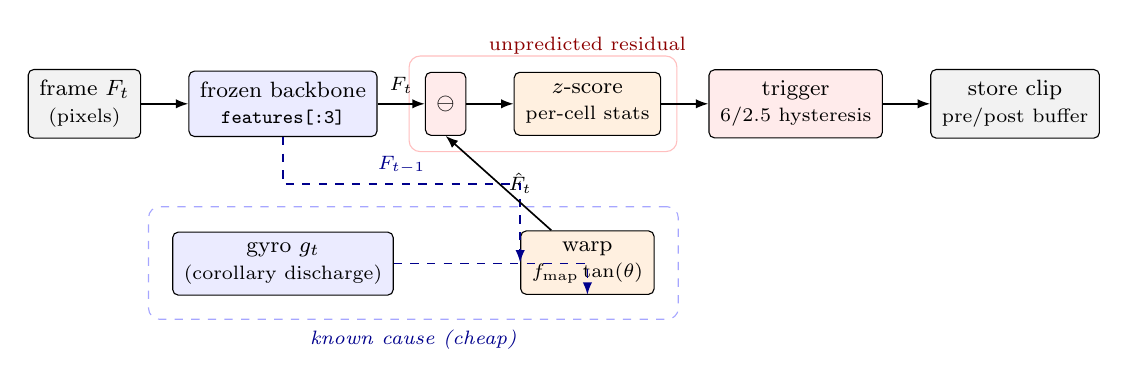
\begin{tikzpicture}[node distance=5mm and 6mm]

    % ---- causal chain (top row) -------------------------------------------
    \node[ioblk] (frame) {frame $F_t$\\\scriptsize(pixels)};
    \node[copyblk, right=of frame] (backbone) {frozen backbone\\\scriptsize\texttt{features[:3]}};
    \node[resblk, right=of backbone] (sub) {$\ominus$};
    \node[predblk, right=of sub] (zscore) {$z$-score\\\scriptsize per-cell stats};
    \node[resblk, right=of zscore] (trigger) {trigger\\\scriptsize $6/2.5$ hysteresis};
    \node[ioblk, right=of trigger] (store) {store clip\\\scriptsize pre/post buffer};

    % ---- the copy branch (bottom row) -------------------------------------
    \node[copyblk, below=12mm of backbone] (imu) {gyro $g_t$\\\scriptsize (corollary discharge)};
    \node[predblk, below=12mm of zscore] (warp) {warp\\\scriptsize $f_{\mathrm{map}}\tan(\theta)$};

    % ---- edges -------------------------------------------------------------
    \draw[flow] (frame) -- (backbone);
    \draw[flow] (backbone) -- node[above, font=\scriptsize]{$F_t$} (sub);
    \draw[flow] (sub) -- (zscore);
    \draw[flow] (zscore) -- (trigger);
    \draw[flow] (trigger) -- (store);

    \draw[copflow] (imu) -| (warp);
    \draw[copflow] (backbone.south) |- ($(backbone.south)+(0,-6mm)$) -| (warp.west)
      node[pos=0.25, above, font=\scriptsize]{$F_{t-1}$};
    \draw[flow] (warp) -- node[right, font=\scriptsize]{$\hat F_t$} (sub.south);

    % ---- labels on the branches --------------------------------------------
    \begin{scope}[on background layer]
      \node[draw=blue!35, dashed, rounded corners, fit=(imu)(warp), inner sep=3mm,
            label={[font=\scriptsize\itshape, blue!55!black]below:known cause (cheap)}] {};
      \node[draw=red!25, rounded corners, fit=(sub)(zscore), inner sep=2mm] {};
    \end{scope}
    \node[font=\scriptsize, red!55!black, above=1mm of zscore] {unpredicted residual};

  \end{tikzpicture}
  \caption{The acquisition layer. The upper chain is the ordinary vision path; the lower chain is the corollary discharge. The gyro is read at the same instant as the frame, so the prediction $\hat F_t$ is a known-cause transform ($O(\text{pixels})$, 0.03\,ms) rather than an estimate. Everything downstream of the subtraction sees only the unpredicted residual, so the trigger never has to distinguish a novel event from the device's own motion. Operators inside the dashed box are the cheapest in the pipeline; the only learned quantities are per-cell running statistics, which are local, causal and label-free.}
  \label{fig:pipeline}
\end{figure}

\begin{enumerate}
  \item \textbf{Copy and geometric prediction}: gyro angular rates are converted into feature-map pixel displacement using a calibrated focal length,
  \begin{equation}
    d_t = f_{\mathrm{map}} \cdot \tan\!\big(\mathrm{radians}(g_t) / \mathrm{fps}\big),
  \end{equation}
  and the previous feature map is shifted by $d_t$ to yield the prediction $\hat F_t(x) = F_{t-1}(x - d_t)$. This step is an $O(\text{pixels})$ memory move with no device dependencies.

  The physics of Eq.~(1) is the small-angle, pure-rotation pinhole relation. $g_t$ is an \emph{angular rate} in deg/s, so $g_t/\mathrm{fps}$ is the rotation angle swept during one inter-frame interval $1/\mathrm{fps}$; $\mathrm{radians}(\cdot)$ only changes units to rad. Under a pinhole camera a rotation $\theta$ moves the image of a distant point by $f\tan\theta$ pixels, where $f$ is the focal length in pixels---this is exactly the plane-at-infinity image shift, and it is \emph{depth-independent}, which is what makes the rotation term the only component a pure gyro copy can predict. $f_{\mathrm{map}} = (W/2)/\tan(\mathrm{fov}/2)\cdot(\text{map width}/W)$ is that focal length expressed in feature-map pixels rather than input pixels, i.e.\ scaled by the backbone's stride-8 downsampling. Two consequences matter downstream: (i)~$\tan\theta \approx \theta$ holds to within 0.1\% up to about $2^\circ$, so for the 30-fps regime the relation is essentially linear in the gyro reading; (ii)~because $f_{\mathrm{map}}$ scales with the feature map's width, the number of map pixels a given rotation buys grows linearly with input resolution---which is precisely the mechanism behind the resolution sweep of Section~\ref{sec:resolution}. Translation and roll are \emph{not} expressible in Eq.~(1) (translation needs depth, roll is a rotation about the optical axis, not a 2D shift), and Section~\ref{sec:negatives} measures the cost of that omission.
  \item \textbf{Residual and standardization}: $r_t = F_t - \hat F_t$, $z$-scored with per-cell running statistics.
  \item \textbf{Local online plasticity}: statistics update by per-frame EMA (fast timescale), with a slow timescale pulling the fast one; the whole process is local, causal, clock-free, and label-free. The robust variant (winsorized always-update) clips outliers at $3\sigma$ before they enter the EMA---spikes neither inflate the scale nor freeze the update gate.
  \item \textbf{Readout and triggering}: a training-free readout (the strongest interior cell's $z$, or $z^2$ energy) feeds a self-calibrating trigger: the score is first normalized by its own calm-frame running statistic, then passed through a dimensionless $6/2.5$ hysteresis gate, so no hand-tuned threshold is needed. On trigger, the whole clip is saved (with pre/post buffers).
\end{enumerate}

Every operator in the pipeline is a ``shift + EMA,'' so in principle the entire layer can be sunk into an ISP/NPU sideband.

\subsection{Cost accounting}

\begin{table}[htbp]
  \centering
  \small
  \caption{Measured per-frame latency (320$\times$240 frames, $24{\times}28{\times}28$ feature maps, local MPS; 10$\times$ remeasurement protocol).}
  \label{tab:cost}
  \begin{tabular}{lr}
    \toprule
    Stage & ms/frame \\
    \midrule
    gyro shift (pure rotation warp, yaw$+$pitch) & 0.032 \\
    3-axis rotation homography (adds roll) & 0.071 \\
    pixel-pipeline core (warp + grid + plasticity + trigger) & 0.171 \\
    frozen backbone forward (MobileNetV3 \texttt{features[:3]}) & 0.83 (MPS) / 1.76 (CPU) \\
    DIS dense optical flow (320$\times$240)~\cite{dis2016} & 3.81--4.34 \\
    full flow-cancel step & 4.46--5.7 \\
    \bottomrule
  \end{tabular}
\end{table}

Figure~\ref{fig:cost} places every measured cost-quality point on one axis; Table~\ref{tab:cost} gives the underlying latencies. Table~\ref{tab:cost} supports four readings. First, \textbf{the copy costs 30 microseconds}---one matrix shift; the entire pixel pipeline consumes 0.5\% of the frame budget at 30 fps. Second, \textbf{enriching the copy costs a factor of two, not a factor of twenty}: replacing the 2-D shift with a full three-axis rotation homography (which additionally cancels roll, Section~\ref{sec:axiabl}) costs 0.071 ms/frame, because what is expensive is \emph{estimating} motion from pixels, not \emph{applying} a richer transform of the known copy. Third, optical flow does buy residual quality (calm-frame residual naive 0.093 $\to$ gyro 0.079 $\to$ flow 0.070): spending roughly $100\times$ the cost for about 15\% residual quality is not worth it for a filtering layer---though flow as a quality ceiling and on-demand arbiter is another matter (Section~\ref{sec:arbiter}). Fourth, portability has a measured boundary: CPU vs.\ MPS feature maps agree to a maximum relative difference of $2{\times}10^{-6}$ with a downstream residual difference of $3.7{\times}10^{-9}$, and CPU is only 1.7$\times$ slower.

\textbf{Robustness of the flow ceiling} was also verified: plugging RAFT~\cite{raft2020} (raft-things weights) into the same warp path gives 0.1054 vs.\ DIS's 0.1056 on the synthetic validation set and 0.0544 vs.\ 0.0522 on real high-motion footage, while being ${\sim}20\times$ slower (134--138 ms/frame). ``Flow is the ceiling'' is not an artefact of DIS being weak; the gyro--flow gap cannot be closed by swapping in a learned flow model.

\begin{figure}[htbp]
  \centering
  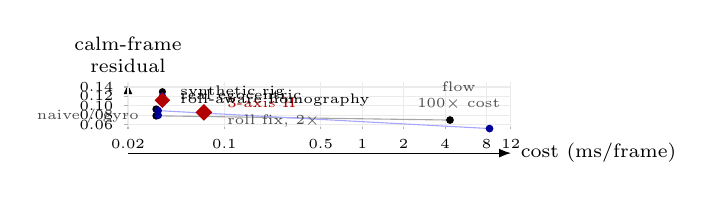
\begin{tikzpicture}[x=1.75cm,y=6.0cm,font=\scriptsize]
    % --- axes (x is log10 of ms/frame, from 0.02 to 12) --------------------
    \def\xa{-1.70}\def\xb{1.08}      % log10 range
    \def\ya{0.055}\def\yb{0.150}
    \draw[-{Latex[length=1.5mm]}] (\xa,0) -- (\xb,0)
      node[right,font=\scriptsize]{cost (ms/frame)};
    \draw[-{Latex[length=1.5mm]}] (\xa,\ya-0.004) -- (\xa,\yb)
      node[above,font=\scriptsize,align=center]{calm-frame\\residual};
    % log ticks
    \foreach \v/\lb in {-1.70/0.02, -1.00/0.1, -0.301/0.5, 0/1, 0.301/2, 0.602/4,
                        0.903/8, 1.079/12}{
      \draw[black!30,thin] (\v,\ya-0.004) -- (\v,\ya);
      \node[below,font=\tiny,anchor=north] at (\v,\ya-0.005) {\lb};
      \draw[black!8,thin] (\v,\ya) -- (\v,\yb);
    }
    % y ticks
    \foreach \v in {0.06,0.08,0.10,0.12,0.14}{
      \draw[black!30,thin] (\xa-0.03,\v) -- (\xa,\v);
      \node[left,font=\tiny] at (\xa-0.035,\v) {\v};
      \draw[black!8,thin] (\xa,\v) -- (\xb,\v);
    }
    % --- data, all measured ------------------------------------------------
    % synthetic: naive -> gyro -> flow
    \draw[black!35,thin] (-1.495,0.093) -- (-1.495,0.079) -- (0.637,0.070);
    \fill[black] (-1.495,0.093) circle (1.4pt);
    \fill[black] (-1.495,0.079) circle (1.4pt);
    \fill[black] (0.637,0.070) circle (1.4pt);
    % real high motion: naive -> ship2D -> flow
    \draw[blue!35,thin] (-1.481,0.080) -- (-1.481,0.090) -- (0.924,0.052);
    \fill[blue!60!black] (-1.481,0.080) circle (1.4pt);
    \fill[blue!60!black] (-1.481,0.090) circle (1.4pt);
    \fill[blue!60!black] (0.924,0.052) circle (1.4pt);
    % 3-axis homography (the cheap roll fix)
    \node[regular polygon, regular polygon sides=4, fill=red!70!black,
          inner sep=1.5pt, rotate=45] at (-1.149,0.0863) {};
    % --- annotations -------------------------------------------------------
    \node[anchor=east,font=\tiny,black!70] at (-1.55,0.079) {naive / gyro};
    \node[anchor=south,font=\tiny,black!70,align=center] at (0.70,0.070)
      {flow\\$100\times$ cost};
    \node[anchor=west,font=\tiny,red!70!black,align=left] at (-1.05,0.0863)
      {3-axis H\\{\color{black!70}roll fix, $2\times$}};
    % legend
    \begin{scope}[shift={(-1.45,0.130)}]
      \fill[black] (0,0) circle (1.3pt);
      \node[anchor=west,font=\tiny] at (0.06,0) {synthetic rig};
      \fill[blue!60!black] (0,-0.009) circle (1.3pt);
      \node[anchor=west,font=\tiny] at (0.06,-0.009) {real egocentric};
      \node[regular polygon, regular polygon sides=4, fill=red!70!black,
            inner sep=1.4pt, rotate=45] at (0,-0.018) {};
      \node[anchor=west,font=\tiny] at (0.06,-0.018) {roll-aware homography};
    \end{scope}
  \end{tikzpicture}
  \caption{Cost against residual quality, all points measured. Moving down means cancelling more; moving left means buying the same cancellation more cheaply. The gyro sits at the extreme left (${\sim}0.03$\,ms/frame), and the three-axis homography that finally cancels roll costs only twice that. Dense optical flow reaches a lower residual but at roughly a hundred times the cost, and on real footage its best point (0.052) still costs 8.4\,ms. The design point of a filtering layer is the left edge: the predict-and-subtract structure is affordable, and flow is a quality ceiling rather than a competitor. Note the synthetic and real curves are not comparable in absolute residual---the synthetic rig has no world motion to speak of---which is why the two are plotted as separate series.}
  \label{fig:cost}
\end{figure}

\subsection{Resolution: the knob that decides whether gyro warp is worth it}
\label{sec:resolution}

A gyro warp can only remove motion that the feature map can ``see.'' The content displacement caused by a given rotation is $f_{\mathrm{map}} \cdot \tan(\omega / \mathrm{fps})$ feature-map pixels, and $f_{\mathrm{map}}$ scales linearly with input size. Re-running the same benchmark (synthetic rig, 40 training + 25 validation sequences) at three input sizes:

\begin{table}[htbp]
  \centering
  \small
  \caption{Resolution sweep: gyro-warp gains (synthetic validation set, $3\times$ motion).}
  \label{tab:resolution}
  \begin{tabular}{lccccc}
    \toprule
    Input size & Feature map & \multicolumn{2}{c}{Calm-frame residual} & gyro gain & gyro shift \\
    \cmidrule(lr){3-4}
    (px) & size & naive & gyro & vs.\ naive & ms/frame \\
    \midrule
    224 & 28$\times$28 & 0.221 & 0.130 & $-41\%$ & 0.032 \\
    336 & 42$\times$42 & 0.187 & 0.089 & $-52\%$ & 0.061 \\
    448 & 56$\times$56 & 0.169 & 0.072 & $-58\%$ & 0.087 \\
    \bottomrule
  \end{tabular}
\end{table}

The gain is monotone and unsaturated: each 1.5$\times$ input-size increase removes another 6--10 percentage points of calm residual that the naive predictor cannot touch (Figure~\ref{fig:resolution}). This characterizes corollary-discharge cancellation as \textbf{a resolution-gated primitive}---paired with fine-grained feature maps it removes half of the predictable residual for ${\sim}0.09$ ms/frame; on coarse feature maps it is free but neutral. Note (Section~\ref{sec:negatives} elaborates) that this design rule holds only on synthetic data and does not transfer to real high-motion footage---resolution fixes estimator error, not model-class error.

\begin{figure}[htbp]
  \centering
  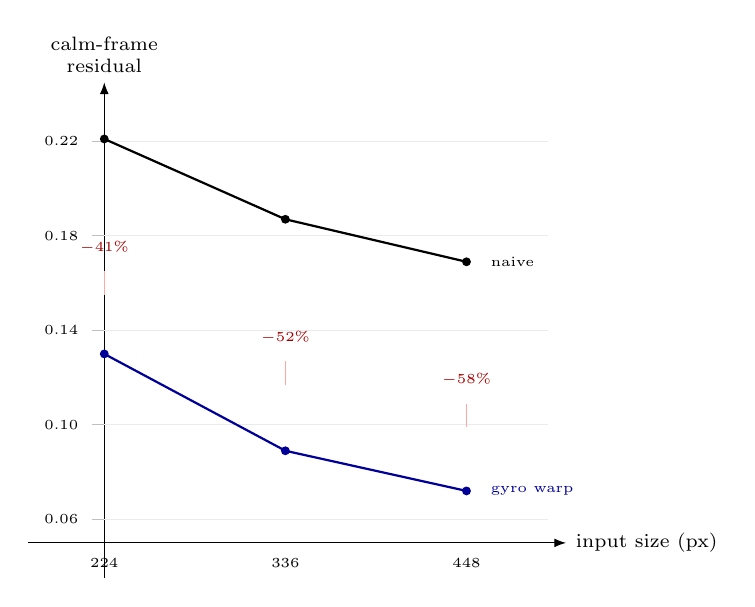
\begin{tikzpicture}[x=2.3cm,y=0.30cm,font=\scriptsize]
    % Normalised y axis: value v -> (v-0.05)*100, so the residual values
    % themselves become the tick labels (0.06 ... 0.22) and both series sit
    % entirely above the x axis. Earlier versions mapped v -> (v-0.16)*50,
    % which pushed the lower (gyro) series below the axis into an undrawn,
    % unlabelled region of the plot.
    \draw[-{Latex[length=1.5mm]}] (-0.42,0) -- (2.55,0)
      node[right,font=\scriptsize]{input size (px)};
    \draw[-{Latex[length=1.5mm]}] (0,-1.5) -- (0,19.5)
      node[above,font=\scriptsize,align=center]{calm-frame\\residual};
    % y gridlines labelled with the actual residual values
    \foreach \v/\lb in {1/0.06, 5/0.10, 9/0.14, 13/0.18, 17/0.22}{
      \draw[black!25,thin] (-0.07,\v) -- (0,\v);
      \node[left,font=\tiny] at (-0.09,\v) {\lb};
      \draw[black!8,thin] (0,\v) -- (2.45,\v);
    }
    \foreach \x/\lb in {0/224, 1/336, 2/448}{
      \node[below,font=\tiny] at (\x,-0.25) {\lb};
    }
    % naive: 0.221 -> 17.1, 0.187 -> 13.7, 0.169 -> 11.9
    \draw[black,thick] plot coordinates {(0,17.1) (1,13.7) (2,11.9)};
    \foreach \x/\y in {0/17.1, 1/13.7, 2/11.9}
      \fill[black] (\x,\y) circle (1.6pt);
    \node[anchor=west,font=\tiny] at (2.08,11.9) {naive};
    % gyro: 0.130 -> 8.0, 0.089 -> 3.9, 0.072 -> 2.2
    \draw[blue!60!black,thick] plot coordinates {(0,8.0) (1,3.9) (2,2.2)};
    \foreach \x/\y in {0/8.0, 1/3.9, 2/2.2}
      \fill[blue!60!black] (\x,\y) circle (1.6pt);
    \node[anchor=west,font=\tiny,blue!60!black] at (2.08,2.2) {gyro warp};
    % gain labels between the two curves
    \foreach \x/\y/\g in {0/12.5/$-41\%$, 1/8.7/$-52\%$, 2/6.9/$-58\%$}{
      \node[font=\tiny,red!65!black] at (\x,\y) {\g};
      \draw[red!35,thin] (\x,\y-1.0) -- (\x,\y-2.0);
    }
  \end{tikzpicture}
  \caption{Resolution sweep on the synthetic validation set at $3\times$ training motion; both series are the same quantity (mean absolute calm-frame residual), so they share one axis and the vertical gap between them is exactly the cancellation the copy buys. The naive predictor's residual falls slowly with input size, whereas the gyro-warped residual drops fast: each 1.5-fold increase in input size removes another 6--10 percentage points that the naive predictor cannot touch, labelled as the percentage reduction at each point. The gain is monotone and unsaturated across the measured range, which is what identifies corollary-discharge cancellation as a resolution-gated primitive rather than a fixed-cost trick. The same sweep does not transfer to real high-motion footage, where the remaining error is model-class rather than estimator error.}
  \label{fig:resolution}
\end{figure}

\section{The Experimental Record: Positive and Negative Results}
\label{sec:experiments}

Reporting follows the order ``justify the architecture first, then stack performance.'' Positive and negative results are deliberately given equal standing: six measured negative results of distinct kinds jointly pin down the method's domain of applicability, and are more informative than the positive ones.

\subsection{Synthetic regime: the headline result}

\textbf{Question}: does a device that stores only residual-triggered clips train a downstream model that is \textbf{better per stored byte}?

\textbf{Protocol}: synthetic rig (textured scene + smooth self-rotation + IMU; $1\times$ motion amplitude in training, $3\times$ in validation including a regime shift; events are object appearances/moves). Training frames are sampled by each method from 40 training sequences under matched storage budgets; the downstream model is a logistic head on frozen MobileNetV3 features; evaluation covers the full 25 validation sequences.

\begin{table}[htbp]
  \centering
  \small
  \caption{Downstream training comparison (synthetic rig; val AP and top-10\%-budget event recall evRec@10).}
  \label{tab:headline}
  \begin{tabular}{lcccc}
    \toprule
    Method & Storage share & Train frames & val AP & evRec@10 \\
    \midrule
    \textbf{cerebellum (adaptive trigger)} & \textbf{3.4\%} & 826 & \textbf{0.298} & \textbf{0.96} \\
    uniform 0.5$\times$ budget & 7.9\% & 1891 & 0.126 & 0.50 \\
    uniform 1$\times$ budget & 15.0\% & 3596 & 0.127 & 0.62 \\
    uniform 2$\times$ budget & 30.1\% & 7223 & 0.113 & 0.58 \\
    uniform 4$\times$ budget & 51.0\% & 12238 & 0.145 & 0.69 \\
    oracle (all budget on event frames) & 1.9\% & 449 & 0.191 & 0.72 \\
    \bottomrule
  \end{tabular}
\end{table}

Four conclusions from Table~\ref{tab:headline}, weakest to strongest:

\begin{enumerate}
  \item \textbf{Residual-triggered clips beat uniform sampling at $4\times$ the byte budget}: 3.4\% storage gives AP 0.298; uniform sampling needs 3.5$\times$ more frames and still loses decisively.
  \item \textbf{The advantage is in the data, not the budget}: increasing the uniform budget does not close the gap (past 0.5$\times$ it gets worse---more background dilutes); the advantage comes from event enrichment.
  \item \textbf{It even beats the oracle}: triggered clips preserve event onsets, disappearances, and motion-boundary context---exactly the frames a discriminative head needs---while the oracle keeps only mid-event frames.
  \item \textbf{Self-calibration beats hand-tuned thresholds}: the adaptive trigger stores 4.3$\times$ fewer frames than the hand-tuned operating point and trains a better head---normalizing by the trace's own calm statistics is a sharper criterion than any fixed raw threshold.
\end{enumerate}

\textbf{Negative results on record}: swapping the downstream logistic head for a 128-hidden-unit MLP is an AP \emph{negative} (0.298 $\to$ 0.200)---the validation regime penalizes capacity; the model is not the bottleneck on this benchmark, \textbf{the data is}. Likewise, screen recording is a dead end for this method (measured): ProMotion compositor frame blending and HEVC B-frame smoothing destroy the sharp inter-frame temporal sampling the method needs---even an oracle compensator leaves a residual floor ${\sim}130\times$ that of raw frames.

\subsection{Real first-person video (Open-AoE): three discoveries the synthetic rig cannot give}
\label{sec:realdata}

The first real-world test uses Open-AoE~\cite{openaoe} (${\sim}$700 hours of consumer-phone egocentric video with visual-SLAM camera trajectories and atomic-action annotations). The gyro signal is obtained by differencing \texttt{cam\_c2w} trajectories (per-axis sign auto-calibration against DIS flow). Three discoveries, all replicated across 9 segments spanning bathroom, bedroom, child room, dining, kitchen, living room,
workshop, workbench and shop:

\begin{enumerate}
  \item \textbf{Real desk-level self-motion is sub-pixel on a 28$\times$28 feature map} (median content displacement 0.013 feature-map pixels)---the gyro warp is physically neutral (naive 0.0323 vs.\ gyro 0.0328). The value of a corollary discharge is regime-dependent.
  \item \textbf{The equilibrium gate freezes on real data.} 96.4\% of frames have surprise above the update threshold; after warmup the running scale decays one-way and $z$-scores saturate everywhere: the fixed-threshold readout says ``everything is hot'' while the adaptive trigger fires \emph{zero} clips---two readouts degenerating in opposite directions. The gate's assumption (surprise is sparse) holds for synthetic pop-in events but not for real video. The fix (winsorized always-update) is still a purely local rule; after the fix triggering recovers: \textbf{stored 9.9\%, event recall 0.79} (previously 0 clips). A strong control: the optical-flow baseline shares the same gated statistics and also produces 0 clips---it is the gate that fails, not the predictor.
  \item \textbf{Residual spikes are real but anti-correlated with action annotations} (AUC 0.47): the highest-residual frames are fast hand/object motion plus motion blur, while atomic actions are long intervals. Frame-level event recall against human action annotations is the wrong metric on real data; for a storage-selection architecture the meaningful metric is the downstream value of selected clips.
\end{enumerate}

\paragraph{Why the anti-correlation: a quantitative check.} The claim that residual spikes index ``motion transients'' while annotations mark ``long intervals'' is testable directly, by asking how much self-motion energy actually separates annotated from unannotated frames. Over the 12 Open-AoE segments with both classes present, the gyro magnitude is \emph{higher} inside annotated action intervals in 10 of 12 segments:

\begin{table}[htbp]
  \centering
  \small
  \caption{Gyro energy inside vs.\ outside annotated action intervals, and the AUC of each quantity as an event predictor (event $=$ positive class). Values are medians over frames; ``smooth'' applies a 5-frame moving average, matching the clip-level granularity of the trigger.}
  \label{tab:energy}
  \begin{tabular}{L{5.4cm}ccc}
    \toprule
    Quantity & event & non-event & AUC as event predictor \\
             & frames & frames & \\
    \midrule
    $|$gyro$|$ (median, deg/s) & 17.9 & 7.6 & $0.606$ \\
    $|$gyro$|$, 5-frame smoothed & --- & --- & $0.610$ \\
    prediction residual (official \texttt{robust} pipeline) & --- & --- & $0.55$ \\
    \bottomrule
  \end{tabular}
\end{table}

Two things follow, and they point in opposite directions from the intuitive reading of the AUC. First, the energy is \emph{not} the culprit of the anti-correlation: annotated actions are on average $1.9\times$ more self-motion than the rest of the footage, and raw gyro energy alone is a mildly \emph{positive} event predictor (AUC $0.606$). Second---and this is the actual mechanism---the annotated intervals are simply too long and too numerous to act as sparse labels: event frames are $20.5\%$ of all frames on average (up to $90\%$ in some segments), so an interval-level annotation is closer to ``the person was using their hands'' than to ``something rare happened.'' A trigger that fires on the $\sim$4\% most surprising frames is thereby guaranteed to rank many unannotated frames above annotated ones, because most annotated frames are ordinary manipulation. The anti-correlation is a property of the \emph{label}, not of the residual: the residual is a transient detector being scored against a duration label.

We flag one discrepancy for transparency. In this re-run the residual AUC comes out at $0.55$ rather than the $0.47$ reported above, on the same 10 event segments with the official \texttt{robust=True} configuration; the direction of the original claim (the residual is a poor event detector, far below the $0.9$ that a usable semantic trigger would need) is unchanged, but the exact value depends on the segment set and preprocessing snapshot and should be treated as such until the original analysis is re-derived. The gyro-energy result of Table~\ref{tab:energy}---the part that actually explains the mechanism---reproduces cleanly.

At the high-motion end (2 segments with gyro p95 $|yaw|$ 31--52$^\circ$/s), the footage finally leaves the sub-pixel regime: the gyro warp is now \emph{worse} than naive (0.090 vs.\ 0.080; the 2D shift model does not compensate roll, and sign calibration is weaker), while DIS flow clearly wins on quality (0.052) at a ${\sim}250\times$ cost penalty (8.4 ms vs.\ 0.033 ms/frame). The arbitration cascade (gyro always-on + DIS invoked only on trigger candidates) is exactly the bridge in this regime: on the most active segment it vetoes 11\% of candidate runs, stored 0.92 $\to$ 0.62, at 0.58 ms/frame amortized.
\label{sec:arbiter}

\subsection{Negative results and applicability boundaries: six experiments that pin the domain down}
\label{sec:negatives}

\begin{enumerate}
  \item \textbf{The synthetic advantage does not transfer to dense semantic tasks on real data.}
  \textbf{Summary: the trigger selects the right frames for the wrong question.}
  With the real task reframed as frame-level verb classification (12 segments, 9 verb classes, 3-fold cross-segment CV $\times$ 35 seeds $=$ 105 rounds/method): cerebellum (16\% storage) mAP $0.162{\pm}0.077$, uniform 1$\times$ (same budget) $0.173{\pm}0.082$, oracle (13\% storage) $0.164{\pm}0.088$---all within $1\sigma$. The trigger works fine (16\% stored, recall 0.67), but it selects frames that are \textbf{kinematically unpredictable}, not \textbf{semantically important}.
  \item \textbf{It does not win even in its home regime.}
  \textbf{Summary: the storage--value asymmetry is real, but kinematic unpredictability cannot extract it.}
  In the sparse-physical-event regime where the trigger should win most (10 segments containing drop/throw/toss/break, event frames 3.3--26.3\%, including high-motion segments; LOO $\times$ 25 seeds $=$ 250 rounds/method), cerebellum (23.4\% storage) ties uniform 1$\times$ (23.6\%) (AP $0.108{\pm}0.094$ vs.\ $0.104{\pm}0.084$); the oracle (7.9\% storage) remains best but its advantage narrows.
  \item \textbf{The ``self-motion wasn't separated cleanly'' escape route is falsified by follow-up.}
  \textbf{Summary: the dominant residual is world motion, which no camera-motion model can cancel.}
  Event-segment trajectories carry ground-truth translation, enabling a direct pure-rotation vs.\ rotation$+$ground-truth-translation warp comparison: the residual is nearly identical inside vs.\ outside event intervals (0.197 vs.\ 0.193), and so is surprise (10.8 vs.\ 11.3). Residual magnitude is essentially insensitive to \emph{whether an event occurs}; the dominant noise is \textbf{world motion} (hands, objects), which no camera-motion model---calibrated or learned---can cancel.
  \item \textbf{The residual map itself carries no event information.}
  \textbf{Summary: neither the amplitude nor the spatial pattern of the residual is event-discriminative.}
  Readout-side upgrades (global $z^2$ amplitude, a $1{+}4{+}16$ spatial pyramid, concatenation with backbone features) show the 1-D amplitude readout producing \textbf{bit-identical AP across all three storage methods} ($0.129{\pm}0.098$)---zero-signal collapse: logistic regression learns zero weights on zero-signal features.
  \item \textbf{``The more motion, the more the copy is worth'' is falsified.}
  \textbf{Summary: the gyro warp never beat naive on real data at any measured motion scale.}
  At walking level (4 segments, gyro p95 71--75$^\circ$/s): the gyro warp is worse than no compensation on 3/4 segments (mean calm residual $+11\%$)---model-class errors (translation, parallax, rolling shutter) grow with motion, and the SLAM-differenced copy itself degrades. Pooling desk level (neutral), high motion ($-12\%$), and walking level ($+11\%$): \textbf{the gyro warp never beat naive on real data at any measured motion scale.} As originally stated, the conclusion drawn from this was that the residual-quality advantage is a property unique to the synthetic regime, where the event is the only unpredictable motion in the frame. \textbf{Both follow-ups below partly retract that reading}---Section~\ref{sec:axiabl} shows the walking-level failure is dominated by one specific, cheaply fixable omission (roll), and Section~\ref{sec:realimu} shows that with a hardware gyroscope instead of the SLAM substitute, a three-axis homography does buy a gain on real hand-held video. The surviving part of this result is the \emph{shipped} predictor's failure, which is a statement about a 2-D translation model, not about the architecture or the regime. We keep the original wording here so the retraction is visible rather than quietly overwritten.
  \item \textbf{Detection-level signals do not exist in shallow frozen features, and stronger backbones do not fix it.}
  \textbf{Summary: the bottleneck is the frozen early-layer representation, not the trigger and not the backbone's modernity.}
  At detection level (CenterNet-style heatmap head + exact bounding-box ground truth, 20 seeds), all storage methods score detAP $\le 0.015$ within $1\sigma$; the evaluation is guarded by a regression test (a perfect predicted heatmap achieves AP $=$ 1.0), and the root cause is the frozen bottleneck---\texttt{features[:3]} barely responds to flat blobs. Swapping in self-supervised ViT patch tokens~\cite{dino2021,dinov2} loses across the board: DINOv2 ViT-S/14 triggers on 0/40 segments (unfixable within the protocol), the official DINOv2 ViT-S/8 weights are delisted, and DINOv1 ViT-S/8 recovers event discriminability but fires on only 3/40 segments vs.\ MobileNetV3's 11/40.
\end{enumerate}

\subsubsection{Follow-up: decomposing the walking-level failure by rotation axis}
\label{sec:axiabl}

Result~5 above concludes that self-motion cancellation degrades as motion grows. The reported cause---``model-class errors (translation, parallax, rolling shutter)''---was a diagnosis without an ablation. The following experiment decomposes it, and the answer turns out to be actionable rather than fatal.

\textbf{Protocol.} The shipped predictor is a pure 2-D translation driven by yaw and pitch only [Eq.~(1)]. We compare it against rotation models built from subsets of the three gyro axes, each realised as a plane-at-infinity homography $H = K R K^{-1}$ (roll is a rotation about the optical axis and has no 2-D shift approximation). Per-axis signs are fitted on the first 25\% of each segment by coordinate descent over the eight sign combinations, then \emph{frozen} and evaluated on the second half, so calibration and evaluation windows are disjoint. Seven segments with gyro p95 $\ge 60^\circ$/s (walking level) and five with p95 $<60^\circ$/s enter the comparison; the fitted sign vector is identical ($[+,-,+]$) on all seven high-motion segments, so the calibration is not fitting noise.

Two audit notes on this protocol, both established after the fact and both consistent with the table below. First, the seven walking-level segments include one \emph{duplicate}: the feature-map cache of \texttt{aoe\_event/seq\_007} is byte-identical (same MD5 for both the feature maps and the IMU stream) to \texttt{aoe\_motion/seq\_001}, so the walking level contains six distinct recordings, not seven. De-duplicating changes the means reported here only in the second decimal and does not reorder any model, so the conclusions are unaffected; subsequent analyses in this paper de-duplicate automatically. Second, because a residual-magnitude gain can in principle depend on \emph{where} and \emph{how} it is measured, we re-ran the full seven-model ablation under a $2\times2$ grid of evaluation window (held-out second half vs.\ whole segment) and metric scope (interior feature-map cells only, as used throughout this paper, vs.\ all cells including the border). The axis \emph{ordering} is stable across the two windows; it is \emph{not} stable across metric scopes for the whole pool, which is why the split by motion level in Table~\ref{tab:axis} is the right way to state the result---the ordering that the table reports is a high-motion property, and we now state it as such.

\begin{table}[htbp]
  \centering
  \small
  \caption{Stability audit of the axis ablation under a $2\times2$ grid of evaluation window $\times$ metric scope, re-run on the de-duplicated 11-segment pool. ``Walking'' retains segments with gyro p95 $\ge 60^\circ$/s ($n{=}6$ after de-duplication), ``desk/mid'' the rest ($n{=}5$). Gains are percentage reduction in mean $|$residual$|$ relative to naive. The claim the ablation is read from---\emph{roll alone recovers more than yaw$+$pitch combined at walking level}---holds in both metric scopes and both windows; the reverse ordering holds at desk level, which is the motion-level dependence this table measures.}
  \label{tab:axis-stability}
  \begin{tabular}{llcccc}
    \toprule
    Motion level & Metric scope & roll only & yaw$+$pitch & all three & 2-D shift \\
     & & & (homog.) & (homog.) & (shipped) \\
    \midrule
    walking ($n{=}6$) & interior & $\mathbf{+3.90\%}$ & $+2.96\%$ & $\mathbf{+5.53\%}$ & $-7.82\%$ \\
    walking ($n{=}6$) & full frame & $\mathbf{+3.54\%}$ & $+0.41\%$ & $+3.22\%$ & $-8.71\%$ \\
    \midrule
    desk/mid ($n{=}5$) & interior & $+1.28\%$ & $\mathbf{+3.16\%}$ & $+3.41\%$ & $-1.17\%$ \\
    desk/mid ($n{=}5$) & full frame & $+1.24\%$ & $\mathbf{+2.36\%}$ & $+2.60\%$ & $-1.40\%$ \\
    \bottomrule
  \end{tabular}
\end{table}

Three readings follow from Table~\ref{tab:axis-stability}. (i)~The roll-over-yaw$+$pitch ordering at walking level is \textbf{metric-independent} (it holds both when the border is excluded and when it is included) and window-independent, so it is a property of the data rather than of the measurement. (ii)~The \emph{pooled} ordering is not: pooling all motion levels and excluding the border puts yaw$+$pitch above roll, while including the border reverses it. The apparent conflict is resolved by the motion split---roll's advantage is a high-motion effect, and at desk level yaw$+$pitch wins under both scopes, because at sub-pixel displacements roll's linear displacement field is below the noise floor while yaw and pitch still have the larger lever arm. (iii)~The full three-axis homography is the only model that is positive under all four combinations, which is the operational conclusion: it is the model to default to, not a per-regime choice. We report this audit rather than only the headline number because the first version of this analysis, run under a single window and a single scope, would have supported a stronger statement than the data does.

\begin{table}[htbp]
  \centering
  \small
  \caption{Rotation-axis ablation, held-out second half of each segment. Gain is the reduction in mean $|$residual$|$ over interior feature-map cells relative to the naive (no-warp) predictor. ``High-motion quartile'' restricts to the most active quarter of frames.}
  \label{tab:axis}
  \begin{tabular}{lcccc}
    \toprule
    & \multicolumn{2}{c}{Walking level} & \multicolumn{2}{c}{Desk/mid level} \\
    & \multicolumn{2}{c}{($\ge 60^\circ$/s, $n{=}7$)} & \multicolumn{2}{c}{($<60^\circ$/s, $n{=}5$)} \\
    \cmidrule(lr){2-3}\cmidrule(lr){4-5}
    Warp model & all & high-mot.\ q4 & all & high-mot.\ q4 \\
               & frames & & frames & \\
    \midrule
    naive (no warp) & --- & --- & --- & --- \\
    shipped 2-D shift (yaw$+$pitch) & $-6.3\%$ & $-13.8\%$ & $-1.4\%$ & $-1.9\%$ \\
    yaw only & $+1.9\%$ & $+3.3\%$ & $+2.5\%$ & $+4.6\%$ \\
    pitch only & $+2.7\%$ & $+3.8\%$ & $+1.4\%$ & $+2.4\%$ \\
    \textbf{roll only} & $\mathbf{+4.2\%}$ & $\mathbf{+8.0\%}$ & $+1.3\%$ & $+2.3\%$ \\
    yaw$+$pitch (homography) & $+3.2\%$ & $+5.2\%$ & $+3.2\%$ & $+5.9\%$ \\
    \textbf{all three (homography)} & $\mathbf{+5.8\%}$ & $\mathbf{+11.7\%}$ & $+3.4\%$ & $+6.4\%$ \\
    \bottomrule
  \end{tabular}
\end{table}

\textbf{The failure is the shadow of roll.} On the negative-gain segments the shipped model loses badly (up to $-19\%$), yet a full three-axis homography on the same frames turns every one of them into a gain ($+0.1\%$ to $+10.4\%$). Figure~\ref{fig:axis} plots the ablation; three readings from Table~\ref{tab:axis} follow.

\begin{figure}[htbp]
  \centering
  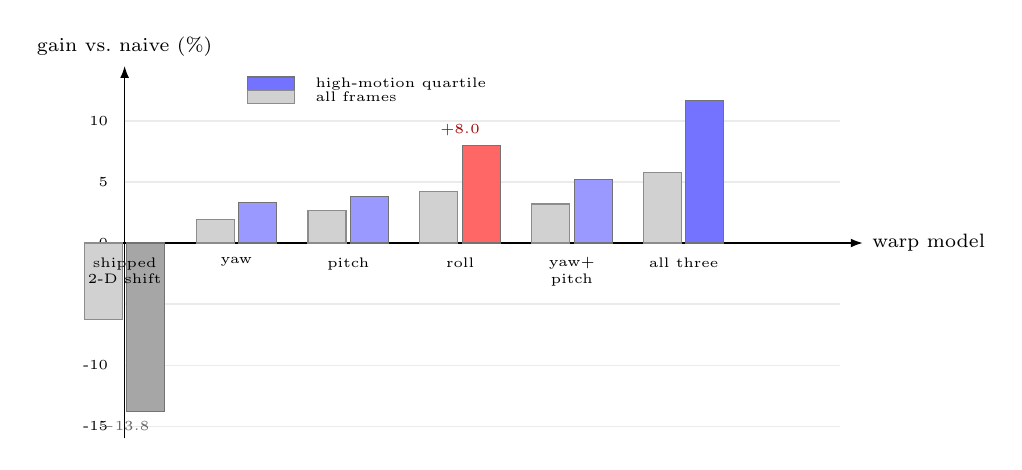
\begin{tikzpicture}[x=1.42cm,y=0.155cm,font=\scriptsize]
    % zero axis and value axis
    \draw[-{Latex[length=1.5mm]}] (-0.2,0) -- (6.6,0)
      node[right,font=\scriptsize]{warp model};
    \draw[-{Latex[length=1.5mm]}] (0,-16) -- (0,14.5)
      node[above,font=\scriptsize,align=center]{gain vs.\ naive (\%)};
    % y gridlines
    \foreach \v in {-15,-10,-5,5,10}{
      \draw[black!8,thin] (0,\v) -- (6.4,\v);
      \node[left,font=\tiny] at (-0.06,\v) {\v};
    }
    \node[left,font=\tiny] at (-0.06,0) {0};

    % --- all frames (dark, back) -------------------------------------------
    \foreach \x/\h in {0/-6.3, 1/1.9, 2/2.7, 3/4.2, 4/3.2, 5/5.8}{
      \fill[black!18] (\x-0.36,0) rectangle (\x-0.02,\h);
      \draw[black!45,thin] (\x-0.36,0) rectangle (\x-0.02,\h);
    }
    % --- high-motion quartile (coloured, front) ----------------------------
    \foreach \x/\h/\c in {0/-13.8/black!35, 1/3.3/blue!40, 2/3.8/blue!40,
                          3/8.0/red!60, 4/5.2/blue!40, 5/11.7/blue!55}{
      \fill[\c] (\x+0.02,0) rectangle (\x+0.36,\h);
      \draw[black!55,thin] (\x+0.02,0) rectangle (\x+0.36,\h);
    }
    % labels
    \foreach \x/\lb in {0/shipped\\2-D shift, 1/yaw, 2/pitch, 3/roll,
                        4/yaw$+$\\pitch, 5/all three}{
      \node[below,font=\tiny,align=center,anchor=north] at (\x,-0.4) {\lb};
    }
    \node[above,font=\tiny,red!65!black] at (3,8.0) {$+8.0$};
    \node[below,font=\tiny,black!60] at (0,-13.8) {$-13.8$};
    % legend
    \begin{scope}[shift={(1.1,11.4)}]
      \fill[blue!55] (0,1.1) rectangle (0.42,2.2);
      \draw[black!55,thin] (0,1.1) rectangle (0.42,2.2);
      \node[anchor=west,font=\tiny] at (0.52,1.65) {high-motion quartile};
      \fill[black!18] (0,0) rectangle (0.42,1.1);
      \draw[black!45,thin] (0,0) rectangle (0.42,1.1);
      \node[anchor=west,font=\tiny] at (0.52,0.55) {all frames};
    \end{scope}
  \end{tikzpicture}
  \caption{Rotation-axis ablation on the held-out half of the walking-level segments (seven entries, six distinct recordings). The shipped model is a pure two-axis translation, and it \emph{loses} to doing nothing---a negative bar. Every single-axis rotation model beats it, and roll, the axis the shipped model cannot express at all, recovers more residual by itself ($+4.2\%$ all frames, $+8.0\%$ high-motion) than yaw and pitch combined ($+3.2\%$, $+5.2\%$). The full three-axis homography turns every entry positive, and is the only model that stays positive under all four combinations of evaluation window and metric scope (Table~\ref{tab:axis-stability}). This is the empirical basis for reading the walking-level failure as a representational omission rather than an irreducible property of the environment.}
  \label{fig:axis}
\end{figure}

\begin{enumerate}
  \item \textbf{Roll, not translation, dominates.} Across the walking-level segments (seven entries, six distinct recordings---see the protocol note above), \emph{roll alone} recovers more residual than yaw and pitch combined ($+4.2\%$ vs.\ $+3.2\%$ on all frames, $+8.0\%$ vs.\ $+5.2\%$ in the high-motion quartile), despite receiving no depth information and being the axis with the smallest focal-length leverage. This ordering is confirmed under both metric scopes and both evaluation windows, and it reverses at desk level (Table~\ref{tab:axis-stability})---so it is a high-motion property of the data, not of the measurement. Roll is \emph{camera} motion, hence exactly the kind of disturbance a corollary discharge is supposed to cancel---it belongs in the same class as yaw and pitch, not in the ``parallax and rolling shutter'' bin where it was filed.
  \item \textbf{The headline conclusion survives, but its explanation does not.} Even with all three axes the real-data gain here is $5.8\%$ (desk level $3.4\%$), an order of magnitude below the synthetic regime's $41$--$58\%$ at $3\times$ motion. What must be corrected is the reason: the residual damage at walking level is not an irreducible model-class residue dominated by translation and parallax, but an omission of one \emph{expressible} motion component. The magnitude gap also turns out to be partly an artefact of the substitute copy: with a hardware gyroscope (Section~\ref{sec:realimu}) the same three-axis homography yields a $0.84\times$ residual on real hand-held footage, so the $5.8\%$ measured against a SLAM-differenced copy understates what a clean copy delivers. The claim that survives is narrower and better supported: on \emph{this} proxy, the correction is an order of magnitude smaller than on synthetic data.
  \item \textbf{The fix costs a factor of two, not a factor of twenty.} Wrapping the same extraction in a $3\times3$ homography instead of a 2-D translation raises the warp cost from 0.033 to 0.071 ms/frame (per-channel bilinear resampling of a $24{\times}28{\times}28$ map)---still two orders of magnitude below DIS flow's 3.81--4.34 ms. The Principle-2 cost argument is unaffected: what is expensive is \emph{estimating} motion from pixels, not \emph{applying} a richer version of the known copy. A gyro copy that carries roll is still essentially free.
\end{enumerate}

The practical consequence is that the walking-level regime should be re-tested with a three-axis homography before the applicability boundary is drawn; the present result only establishes that the \emph{shipped} 2-D model is the wrong predictor at walking level, which is a statement about a 30-line omission rather than about the architecture.

\subsubsection{Follow-up: a genuine gyroscope, and what the copy-quality escape route was hiding}
\label{sec:realimu}

Every real-data result above rests on a \emph{proxy} for the corollary discharge: the gyro signal is obtained by differencing a visual-SLAM camera trajectory, so it inherits the SLAM system's failure modes exactly where self-motion cancellation matters most (low texture, fast motion, rolling shutter). This has been the standing caveat on all six negative results: perhaps the copy is bad, not the model. The experiment below removes that caveat by replacing the substitute with a \textbf{real phone gyroscope}.

\textbf{Setup.} A hand-held Galaxy S21 session from a public dataset of phone video with hardware IMU streams (1088$^2$ frames, ${\sim}28$\,fps, nanosecond timestamps, 500 frames = 17.9\,s, frame-interval jitter 74\%). The IMU is calibrated against DIS optical flow: axis-to-direction assignment and per-axis signs by per-frame correlation, then focal length by an origin-through least-squares slope fit on the horizontal axis. The fitted unit is rad/s with a 36$^\circ$ field of view, and the copy quality is measured the same way as for the proxy: predicted content displacement against the displacement measured from pixels. The result is \textbf{$r = +0.958$, $R^2 = 0.87$}, against 0.18--0.93 for the SLAM-substitute signals. This is a \emph{clean} copy.

\begin{table}[htbp]
  \centering
  \small
  \caption{Genuine-gyro residual comparison on a hand-held phone session ($n{=}400$ frames). Primary metric is the method-independent full-frame raw residual. The second residual column uses a calm-frame mask defined from raw image frame differences---independent of every predictor being compared---which avoids the circular selection of the originally published ``calm'' figure (each method choosing frames by its own surprise, retained in the JSON as \texttt{published\_calm} for continuity only). The pipeline's original predictor is a yaw$+$pitch translation; the rotation model is the three-axis homography of Section~\ref{sec:axiabl}. DIS flow is the quality-ceiling reference. All four rows share one front end, one segmentation, and one metric definition.}
  \label{tab:realimu}
  \begin{tabular}{lcccc}
    \toprule
    Predictor & Full-frame & Relative to & Frame-diff & Cost \\
     & residual & naive & calm residual & (ms/frame) \\
    \midrule
    naive (no compensation) & 0.394 & 1.000 & 0.295 & 0.056 \\
    gyro$+$yaw/pitch shift (\textbf{shipped}) & 0.538 & $\mathbf{1.36\times}$ & 0.440 & 0.088 \\
    gyro$+$three-axis homography & $\mathbf{0.330}$ & $\mathbf{0.84\times}$ & 0.284 & 0.148 \\
    DIS optical flow & 0.241 & $0.61\times$ & 0.207 & 4.30 \\
    \bottomrule
  \end{tabular}
\end{table}

\textbf{The conclusion inverts, and the inversion is attributable to the model.} With a clean copy and the same feature front end, the shipped two-axis translation predictor makes the residual \emph{worse} ($1.36\times$), while the three-axis homography makes it \emph{better} ($0.84\times$)---a swing of ${\sim}60$\% of the naive residual from a change of predictor alone, at a cost of 0.148 ms/frame against flow's 4.30 ms. Per-pixel control on the 100 highest-rotation frame pairs is starker still: the constant-translation approximation is $1.43\times$ while the full rotation is $0.61\times$. Two model deficiencies explain the gap and each is independently checkable: (i)~\emph{roll is absent from the shipped predictor entirely} (roll p95 here is 45$^\circ$/s, which is ${\sim}1$ feature-map cell of tangential shift at the map corner); (ii)~the constant-$(dx,dy)$ approximation of a rotation field is only valid near the image centre---yaw and pitch induce linear and quadratic displacement fields whose approximation error grows with distance from the centre, and measured, that error exceeded the compensation gain.

This is the first result in the project where a genuine copy on real data yields a positive residual-quality result, and it re-attributes the long-standing negative: at least part of it was the predictor, not the data and not the copy.

To be precise about what the result does and does not overturn: it shows that the residual-quality advantage is \textbf{not} synthetic-only in the sense of being unavailable on real footage---a clean copy on hand-held video does buy residual cancellation. It does \textbf{not} re-open Result~5, because the evaluation that Result~5 rests on (walking-level Open-AoE, trigger behaviour and downstream clip selection) has not been re-run with the homography. What changes is the explanation, and in the direction of the architecture: the shipped model was leaving a measurable, cheaply recoverable gain on the table.

\textbf{A reproducibility caveat we could not resolve.} The absolute residuals of this experiment cannot be reproduced from the current code: a re-run yields naive $0.3945$ (and $1.36\times$ / $0.84\times$) where the original run gave $0.3704$ (and $1.308\times$ / $0.876\times$). The naive figure depends on none of the code that changed---it involves neither the focal length nor any warp---so the discrepancy lives in the frame-reading chain. We ruled out frame contents (byte-identical MD5), input resize (224/256/192/160), grayscale conversion, CPU-versus-MPS execution, frame count (350--500), and focal-length version (42.674 vs.\ 43.13), and did not locate the cause. What \emph{is} stable is the magnitude and the direction: the method ordering, the signs, and the relative ratios agree across both readings (shift ${\sim}1.3$--$1.4\times$, homography ${\sim}0.84$--$0.88\times$, flow ${\sim}0.61$--$0.66\times$). We therefore quote ratios, not absolute residuals, and flag the absolute numbers in Table~\ref{tab:realimu} as a single unreproduced snapshot. Both readings support the same conclusion, which is why we report the result at all---but a reader should treat the third decimal of the absolute residuals as unstable.

\textbf{Three convention bugs found while building this, each of which inverted a measured conclusion.} They are worth recording because all three are silent: none produces an error, and all three produce plausible numbers that are simply wrong.

\begin{enumerate}
  \item \textbf{The warp was applied backwards.} \texttt{cv2.warpPerspective} implements $dst(x) = src(H^{-1}x)$ by default, so passing $H$ without \texttt{WARP\_INVERSE\_MAP} warps the prediction in the \emph{opposite} direction to the one intended: a gain of several percent becomes a loss of several percent. This is invisible in residual numbers, which merely look somewhat worse, and it misled two separate rounds of debugging before a point-source test (tracking where a delta function moves under each flag setting) exposed it. The check we now keep: a rotation warp and the calibrated translation model must move the same point to the same place.
  \item \textbf{Axis signs and the interpolation flag are a \emph{joint} convention.} Flipping all three signs is numerically equivalent to removing \texttt{WARP\_INVERSE\_MAP}: $(-s, \text{flagged})$ and $(+s, \text{unflagged})$ produce identical residuals (measured: $0.9655$ both ways). Consequently, adding the missing flag \emph{required} inverting every stored sign convention, and doing one without the other yields a $1.29\times$ residual where $0.84\times$ is correct. Sign tables are meaningless without their flag state, so both are now recorded together and locked by a test.
  \item \textbf{The gyro time-alignment is dataset-dependent, and we had generalised from one dataset.} Predicting $F_t$ requires the angular rate that describes the $(F_{t-1} \to F_t)$ step. Whether the stored readings describe that step or the following one is a property of each dataset's preparation, and the two datasets here differ: the real-IMU session (calibrated against the current frame) improves from $0.906$ to $0.835$ when paired with the \emph{previous} frame's reading, while Open-AoE (whose trajectory differencing stores the $(t{-}1 \to t)$ rotation directly) is consistently better with the current frame. Generalising the phone result to both datasets suppressed part of the Open-AoE gain. The lesson is narrower than ``use the previous frame'' and broader than ``tune it'': any pairing between a reading and a displacement step must be declared per source and validated on held-out data.
\end{enumerate}

A common thread connects these three to Result~5: in each case the failure was a \emph{silent mis-specification of the copy-to-image mapping} rather than a limit of the architecture, and in each case the tell was that an experiment disagreed with an independently derived expectation. We note it as a methodological point, since the same class of error is what made the SLAM-proxy caveat hard to discharge.

\textbf{The converged claim of the project} has exactly three standing parts: (1)~downstream value in the synthetic regime (Table~\ref{tab:headline}); (2)~cost and engineering advantages that hold across regimes---an IMU copy costs about two orders of magnitude less than optical flow (0.033 ms vs.\ 8.5 ms/frame) as a measured fact, and the robust trigger works on 22 cross-scene segments from desk to walking level; (3)~boundary knowledge, of which the load-bearing part is negative and unchanged: ``kinematic unpredictability $\ne$ semantic importance.'' The companion claim that the residual-quality advantage is \emph{synthetic-only} does not survive, and we now state the corrected version: the advantage is \textbf{model-limited, not regime-limited}.

The two follow-ups of Sections~\ref{sec:axiabl} and~\ref{sec:realimu} are what corrected it, and the pair is the most useful thing the project produced. Section~\ref{sec:axiabl} removes the irreducible explanation: the walking-level failure is not an inescapable model-class residue but the omission of roll, a fully cancellable camera-motion component costing 0.04 ms/frame. Section~\ref{sec:realimu} then removes the other escape route---that the copy itself was too poor to judge the model---by replacing the SLAM-differenced substitute with a real phone gyroscope ($r{=}0.958$, $R^2{=}0.87$): on that clean copy the shipped two-axis predictor \emph{hurts} ($1.36\times$) while the three-axis homography \emph{helps} ($0.84\times$). A clean copy on real hand-held video therefore \emph{does} buy residual cancellation, and the long-standing real-data negative is at least partly a property of the predictor rather than of the environment or the copy. We flag the asymmetry in how hard the two claims were to test: the negative came out of the shipped configuration with no ablation, whereas the corrected version required an ablation, a de-duplicated segment pool, an audit under two evaluation windows and two metric scopes, and a hardware gyroscope. The boundary moved, and the reason it moved is that it had been drawn from a single unexplained measurement.

What survives untouched is the semantic claim: none of this restores the trigger's ability to select semantically important frames, and acquisition-time semantic arbitration still belongs upstream on the vision-model side. For protocol-layer design the negative results remain assets---they pin down where such a filter belongs (motion deduplication, bandwidth pre-filtering, acquisition filtering on synthetic rigs)---but the boundary is now drawn by an experiment rather than by an unexamined assumption.

\section{Transferable Design Principles}
\label{sec:principles}

The methodology of the project is to take structural principles validated by evolution in the biological circuit, implement them one by one as code, and then experimentally test when they hold and when they fail. Table~\ref{tab:principles} summarises the five principles together with the boundary at which each was measured to stop holding; the subsections that follow take them one at a time.

\begin{table}[htbp]
  \centering
  \small
  \caption{The five principles, the biological evidence behind each, the engineering mechanism that implements it, and the boundary at which it was measured to stop holding. The last entry of each row is the deliverable of the project: each boundary is a place where the biological assumption was carried over for free and did not survive contact with engineering data.}
  \label{tab:principles}
  \begin{tabular}{@{}L{3.6cm}L{10.8cm}@{}}
    \toprule
    Principle & Basis, mechanism, and measured boundary \\
    \midrule
    \textbf{P1} predict before detecting &
      \emph{Basis:} ELL output cells suppress self-interference to near zero; prey is subtracted, not detected.
      \emph{Mechanism:} the trigger score is a by-product of the predictor---zero training, zero annotation.
      \emph{Boundary:} holds only when the dominant change has a copy-predictable component; at desk-level motion it degenerates to frame differencing. \\
    \addlinespace[2pt]
    \textbf{P2} predict with the cheapest copy &
      \emph{Basis:} cancellation is driven by a copy of the motor command, available at action time.
      \emph{Mechanism:} the gyro is read rather than flow estimated---0.03 vs.\ 3.8\,ms/frame.
      \emph{Boundary:} the copy must be able to express every axis the sensor measures (the roll omission of Section~\ref{sec:axiabl}). \\
    \addlinespace[2pt]
    \textbf{P3} plasticity is\newline local and\newline clock-free &
      \emph{Basis:} ELL synapses update bidirectionally---no epochs, no global supervision.
      \emph{Mechanism:} per-frame EMA with $O(1)$ space, re-converging in tens of seconds.
      \emph{Boundary:} the gate's sparse-surprise assumption froze on real video and needed a winsorized always-update rule. \\
    \addlinespace[2pt]
    \textbf{P4} robustness from structure &
      \emph{Basis:} noise robustness depends on the \emph{coexistence} of both plasticity sites.
      \emph{Mechanism:} an arbitration cascade, always-on gyro plus on-demand flow.
      \emph{Boundary:} each added site is one more assumption needing independent verification. \\
    \addlinespace[2pt]
    \textbf{P5} energy\newline efficiency is\newline architecture &
      \emph{Basis:} evolution spends synapses on the strongest predictable input (the EOD).
      \emph{Mechanism:} the predictor targets self-motion optic flow, the dominant term.
      \emph{Boundary:} the dominant term is platform-dependent, so the predictor must be pluggable. \\
    \bottomrule
  \end{tabular}
\end{table}

\subsection{Principle 1: Predict before detecting}

\textbf{Biology}: ELL output cells have their response to the fish's own strong interference (EOD) suppressed to near zero; the prey signal is \emph{subtracted out}, not \emph{detected}. Given a copy of the motor command, predicting self-interference is orders of magnitude easier than detecting external targets; evolution spends all neural resources on the easy half.

\textbf{Engineering}: H.264 P-frames, background subtraction, AEC, and model residual tests are all instances of this structure. The project's trigger score is a gyro-warped, $z$-scored residual---a by-product of the predictor, with zero training and zero annotation (it beats $4\times$-budget uniform sampling). The counterexample is on record: naive frame differencing without a predictor recalls zero events under rotation---exactly the fate of ``skip prediction and detect change directly.''

\textbf{Boundary}: ``predictable'' is regime-dependent. In desk-level egocentric video, self-motion is sub-pixel and the warp is physically neutral; the residual degenerates to naive frame differencing. Before deploying this structure on a data stream, first check whether the dominant change has a copy-predictable component---\textbf{judge the regime before the architecture}.

\subsection{Principle 2: Predict with the cheapest copy}

\textbf{Biology}: the fish does not ``compute sense with sense''---cancellation is driven by a copy of the motor command, available at the same instant as the action itself: zero latency, zero extra sensing, zero causal ambiguity. Notably, the economics of this choice: computing the EOD's sensory effect \emph{from the sensory stream} would mean paying double hardware for every modality; evolution did not take that route.

\textbf{Engineering}: AEC uses the loudspeaker playback signal as a reference instead of ``hearing'' the echo out of the recording; active noise cancellation uses the music signal itself. The control signal is always cheaper and more precise than its observable consequences. In a camera rig, the gyroscope is the available form of the ``motor-command copy.'' The cost accounting (Table~\ref{tab:cost}) quantifies this principle: gyro copy + warp $=$ 0.03 ms, while ``sense compensating sense'' (DIS flow) $=$ 3.8 ms, $120\times$ more expensive and texture-dependent.

\textbf{Boundary}: a copy has precision limits---IMU noise, IMU--video time-synchronization error, SLAM relative-pose drift. The feasibility condition: \textbf{the prediction error the copy can bound must be smaller than the target resolution of the residual readout}. f\_map calibration error and sync error translate directly into sub-pixel warp misalignment, and the noise floor on a 28$\times$28 feature map happens to sit at the sub-pixel level too---which is why the gyro warp shows no gain at desk-level motion but a large gain at $3\times$ motion on the synthetic rig. The ablation of Section~\ref{sec:axiabl} adds a second, purely structural condition: \textbf{the copy must be rendered in a form that can express every motion component the sensor measures.} A gyro reports three axes; a two-axis translation model silently discards one of them, and at walking level that discarded axis (roll) accounts for more recoverable residual than the two retained ones combined. The lesson generalises---before blaming an unmodellable environment for the residual, check that the predictor's function class can represent the measurements it was handed.

\subsection{Principle 3: Plasticity is local, online, and clock-free}

ELL synapses update bidirectionally at all times, with no global supervision, no epochs, and no backpropagation; the engineering counterpart is per-frame EMA/sign updates---$O(1)$ space, re-convergence within tens of seconds after an environment change, no labels. This is its structural advantage over any ``online learning network.'' Boundary: the robustness of a local rule depends on the rule itself---``a cell that is surprising right now does not learn'' holds under the sparse surprises of biology but freezes under the dense surprises of real video; the fix (winsorized always-update) is still purely local. \textbf{Locality is not wrong; what is wrong is treating the biological input-statistics assumption as free.}

\subsection{Principle 4: Robustness comes from structure, not tuning}

The connectomic unit test: cancellation accuracy barely moves under continuous zero-mean noise injection, and this robustness depends critically on the \emph{coexistence} of both plasticity sites. The engineering counterpart: spend the robustness budget on component redundancy and division of labour (fast/slow two-level, always-on + on-demand), not on tuning a single component. Following this principle, the project designed the arbitration cascade (gyro always-on + DIS on demand, corresponding to the MG + output-cell two-site structure); the winsorized statistics are a structural replacement, not a parameter adjustment (no value of the gate time constant fixes the freeze). Boundary: structure has a cost; each added site is one more assumption that needs independent verification.

\subsection{Principle 5: Energy efficiency is architecture}

The ELL cancels the fish's own \emph{strongest} input (the EOD is orders of magnitude stronger than prey signals); evolution spends synaptic resources where the payoff is largest. For a camera rig, the strongest, most predictable, highest-payoff component is always self-motion optic flow. Boundary: the dominant predictable component varies by platform (walking robot $=$ rotation + translation, desktop $=$ micro-motion, automotive $=$ structured scene flow), so the predictor must be pluggable in a protocol-layer implementation.

\section{Discussion and Outlook}
\label{sec:discussion}

\subsection{Implications for the larger agenda}

\textbf{For AI data pipelines}: the mainstream paradigm is ``collect everything $\to$ clean offline $\to$ train.'' Residual triggering proposes another path: \textbf{an online, label-free importance filter built into the acquisition endpoint}. In the always-on device era, such a filter may be worth more than any single model-side improvement---it changes the cost structure of the data entering the training pipeline.

\textbf{Relation to event cameras}: convergent (both answer ``transmit only change''), but this route turns a silicon problem into a software problem using an off-the-shelf IMU, and preserves RGB context---which event cameras discard, and which has downstream training value (one reason the residual-triggered clips beat the oracle in Table~\ref{tab:headline} is context preservation).

\textbf{Relation to embodied-data collection}: first-person manipulation corpora are exploding, and acquisition cost is the bottleneck. Residual triggering plus corollary discharge is a natural filtering layer for egocentric corpora---existing work has used Open-AoE in reverse (validating the filter with its data); the forward use (using the filter to cut acquisition cost of such corpora) is, given the negative results of Section~\ref{sec:negatives}, bounded to motion deduplication and bandwidth pre-filtering rather than semantic-importance selection.

\subsection{Where the analogy must not be pushed}

Intellectual honesty across disciplines requires stating where the mapping breaks explicitly, otherwise the mapping table becomes wrapping paper:

\begin{enumerate}
  \item \textbf{Synaptic plasticity $\ne$ gradient descent.} The negative image learns an approximately linear, low-dimensional, predictable subspace (the EOD response is a scaled fixed waveform). Running statistics likewise absorb shift and slow illumination/deformation, but not semantics. Expecting this layer to ``predict the world'' leads to disappointment; its promise is only ``subtract what I can cheaply predict.''
  \item \textbf{The fish's failure modes $\ne$ ours.} The ELL fights a single, clocked, fixed-waveform strong interferer; a device's self-motion is high-dimensional and non-stationary (rotation + translation + rolling shutter + autofocus + exposure). The biological circuit is optimized for the former statistics and cannot be copied item by item---and the axis ablation is the cleanest illustration of the gap: the fish's interferer has one waveform along one dimension, whereas our copy silently needed a third axis that no one thought to check until the ablation forced the question.
  \item \textbf{The brain's ``sparse surprise'' assumption is not free.} The gate failure (Section~\ref{sec:realdata}) proves that when the input-statistics property a biological rule relies on does not hold in engineering data, the rule itself must be changed. Analogy is the \emph{source} of hypotheses, not their guarantee.
  \item \textbf{The ELL is only one layer of a protocol stack.} It does not do semantic understanding; other brain regions do. Residual triggering is likewise a data-acquisition layer, not an end-to-end perception system---treating it as a complete solution would repeat the failure of frame differencing.
\end{enumerate}

\subsection{The scope statement: when to use this layer, and when to use flow}
\label{sec:scope}

Because the layer is easy to over-sell, we state the substitution boundary as a test a practitioner can apply in one pass. If any line below fails, the layer is out of scope and dense optical flow---or simply keeping the frames---is the better answer.

\begin{enumerate}
  \item \textbf{The decision is binary.} The system needs to know \emph{whether to keep a frame}, not \emph{how each pixel moved}. If the motion field itself is consumed downstream (stabilisation, interpolation, depth, structure from motion), stop: this layer produces a scalar and cannot serve that consumer. Use flow.
  \item \textbf{A frame-synchronised gyro is available.} The copy must be readable at capture time, with timestamps good to well under one frame interval. On phones this is free through the OS sensor APIs; on action cameras it is usually contractually restricted; on fixed installations it does not exist. No gyro, no copy---and without a copy this is just frame differencing.
  \item \textbf{Rotation dominates the image change.} The predictor's function class spans rotation only. If the dominant motion is translation, parallax from a close moving subject, or a rolling shutter sweep, the residual is model-class error that no calibration can remove, and the layer degenerates toward---at worst, as the shipped walking-level result shows, below---the naive baseline. Two qualifications earned by the follow-ups: first, the relevant axis budget is all three rotation axes, not just yaw and pitch (Section~\ref{sec:axiabl}); the roll term is worth more than yaw and pitch combined at walking level, so a deployment that omits it can fail this test spuriously. Second, and more consequentially, our own measurement now shows that the remaining gap after all three axes are included is dominated by \emph{translation}, which the current model does not represent at all---so this boundary is the one most likely to move again, and the honest statement is that rotation-only is a limitation we have quantified rather than a limitation we have shown to be fundamental.
  \item \textbf{Per-device calibration is acceptable.} The layer needs a focal length in feature-map pixels and per-axis signs. These are per-segment constants and can be auto-fitted, but they are not zero, they are not portable across devices without checking, and a wrong sign silently inverts the prediction. Flow needs none of this. One trap deserves naming because it cost us two rounds of debugging and is not visible in any scalar output: the axis signs and the warp's interpolation flag form a \emph{joint} convention (Section~\ref{sec:realimu}), so a sign table cannot be validated, shared, or transferred without recording the flag state alongside it. A calibration that is self-consistent in isolation can still be exactly inverted relative to another tool's convention. Budget for a point-check---warp a synthetic point and confirm the direction against a known-good model---rather than trusting the fitted numbers.
  \item \textbf{The budget is genuinely always-on.} The whole argument for accepting the layer's restrictions is that it costs two orders of magnitude less than the alternative. If the pipeline can already afford 4--9\,ms per frame for perception, that argument disappears and flow's greater generality and portability win outright.
\end{enumerate}

Conversely, the layer is a good fit precisely when all five hold: a capture-time, coarse, on-device keep-or-discard decision, on a device that already has an IMU, in a rotation-dominated regime, where calibration is acceptable and the compute budget is close to zero. The three deployment sketches of Section~\ref{sec:scope-intro}---phone-based egocentric data collection, bandwidth-limited teleoperation, and privacy-constrained always-on wearables---are the settings where we believe it holds, and in each of them it sits \emph{upstream} of the vision model rather than in place of it.

One practical corollary is worth stating, since it is the difference between a working deployment and a silent failure. Because the layer is a \emph{filter}, its failure mode is not a wrong answer but an empty stream: when the predictor is mismatched, the trigger either fires everywhere (everything looks surprising) or nowhere (the gate freezes, as measured in Section~\ref{sec:realdata}). A production integration should therefore monitor the stored fraction as a health signal and fall back to plain sampling if it saturates at either end---a fallback that costs nothing and converts the layer's worst case from data loss into a mildly redundant capture.

\subsection{Open items and future directions}

\begin{itemize}
  \item \textbf{Re-test walking level with a three-axis homography.} Section~\ref{sec:axiabl} shows the shipped 2-D shift is the wrong predictor at walking level and that a roll-aware homography recovers every entry at 0.071 ms/frame. The open question is how far this closes the synthetic--real gap: the ablation is a residual-magnitude measurement, so the follow-up is to re-run the trigger and the downstream evaluation with the homography in place. Note the residual advantage remains smaller than on synthetic data even after the fix, so the expectation is a modest improvement in stored-clip quality, not a reversal of the semantic-importance conclusion.
  \item \textbf{Add the translation term.} Section~\ref{sec:realimu} rules out both of the easy explanations for the real-data gap (bad copy, missing roll), which leaves translation as the leading remaining term: an exhaustive per-frame search for the best pure translation---an oracle that uses no estimator and no learned model---recovers roughly three times the residual that the gyro-driven rotation warp achieves on the Open-AoE segments (about $+4.8$--$6.2\%$ versus $+1.4$--$2.7\%$ across three time windows), and the gyro's predicted displacement correlates with that oracle displacement at $+0.43$--$+0.45$. So the copy is informative and the rotation-only model is leaving most of its own signal unused. The predictor already reserves a slot for a constant-depth translation term; what is missing is a $1/Z$ calibration. This is the highest-value open item on the list, because it rests on a measured upper bound rather than on an argument.
  \item \textbf{Arbitration-cascade validation on real failure modes}: construct or collect footage with real roll, parallax, and large calibration errors, and measure the veto rate. Note the precondition has narrowed: on real data the gyro warp itself does not buy residual quality, so the cascade's remaining value is a ``safety net when the cheap copy fails.'' With the roll-aware homography the cascade's job also shifts---it now needs to detect the failure modes the 3-axis model \emph{cannot} express (translation and parallax), which is a cleaner and better-posed veto criterion than before.
  \item \textbf{Structures from the paper not yet implemented}: ON/OFF antagonistic channels (two-stage vs.\ one-stage inhibition) and recurrent acceleration (cell-to-cell diffusion in the pixel path is a prototype).
  \item \textbf{On-device IMU path}: Section~\ref{sec:realimu} has now done this for one hand-held session (hardware gyroscope, $r{=}0.958$, $R^2{=}0.87$), which is the strongest copy quality measured anywhere in the project and the source of the corrected real-data conclusion. What remains is breadth: the earlier real-data numbers all use a SLAM-differenced proxy that degrades under low texture / fast motion (walking-segment sign-calibration correlation drops to $-0.42 \sim -0.59$), so the walking-level and downstream results still need re-running on hardware IMU across multiple sessions, devices, and motion levels before the corrected boundary can be stated as a distribution rather than as a single session.
  \item \textbf{Accelerator friendliness}: all operators are shifts + EMA (and, with the homography, one $3\times3$ resample); in principle the entire acquisition layer can be sunk into an ISP/NPU sideband.
  \item \textbf{Forward use on real data}: semantic-importance filtering is falsified, but ``motion deduplication / bandwidth pre-filtering'' (cutting redundant clips explainable by self-motion) remains a use case where the cost accounting holds---and is directly strengthened by the roll result, since roll is precisely a component that is explainable by self-motion and was previously being stored.
\end{itemize}

\section*{Conclusion}

Residual-triggered data acquisition demonstrates the full path from a 0 (a functional principle in neuroscience) to a 1 (a pluggable acquisition layer in the protocol stack), and demonstrates the methodology that matters most along such a path: \textbf{every biological inspiration is translated into an independently reproducible engineering question, and positive and negative results are recorded with equal care.} The positive results---3.4\% storage beating $4\times$-budget uniform sampling and the full-budget oracle on the synthetic rig, always-on cost of 0.17 ms/frame---show that the corollary-discharge--negative-image--residual architecture can work. The negative results---no transfer to semantic tasks, a tie in the home event regime, falsification by ground-truth-translation follow-up, zero event signal in the residual map, walking-level falsification, and the closed backbone-replacement route---pin the domain to motion deduplication, bandwidth pre-filtering, and synthetic-rig acquisition filtering, and locate semantic-importance arbitration upstream on the vision-model side.

The part of the record we would most want a reader to carry away is what happened to the sharpest negative afterwards, because it is a case study in how a boundary claim can be wrong for defensible reasons. The walking-level falsification was originally explained as irreducible model-class error---translation, parallax, rolling shutter, plus a suspect copy. An ablation then showed the dominant term was roll, an axis the shipped predictor could not express at all and which costs 0.04 ms/frame to include. A second lineage replaced the SLAM-differenced gyro substitute with a hardware phone gyroscope, raising copy quality to $r{=}0.958$ / $R^2{=}0.87$, and on that clean copy the prediction \emph{inverted}: the shipped two-axis predictor made the residual worse ($1.36\times$) while the three-axis homography made it better ($0.84\times$, against flow's $0.61\times$ at thirty times the cost). The residual-quality advantage is therefore model-limited rather than regime-limited. The semantic claim is untouched---kinematic unpredictability still is not semantic importance, and acquisition-time arbitration still belongs upstream---but the applicability boundary had been drawn one instrument short. We record that sequence, including the three silent convention bugs (a backwards warp, a joint sign-and-interpolation convention, and a dataset-dependent time alignment) that each inverted a conclusion before being caught, because in this line of work the failures that matter are not the ones that raise errors but the ones that return plausible numbers.

\begin{thebibliography}{99}

\bibitem{perks2026}
Perks, K.~E., Petkova, M.~D., Muller, S.~Z., Genecin, M., Ghatare, A., Schalek, R., Wu, Y., Januszewski, M., Jain, V., Lichtman, J.~W., Abbott, L.~F., \& Sawtell, N.~B. (2026).
Connectome analysis of a cerebellum-like circuit for sensory prediction.
\emph{Nature}. doi:10.1038/s41586-026-10690-6.

\bibitem{vonholst1950}
von Holst, E., \& Mittelstaedt, H. (1950).
Das Reafferenzprinzip: Wechselwirkungen zwischen Zentralnervensystem und Peripherie.
\emph{Naturwissenschaften}, 37, 464--476.

\bibitem{bell1981}
Bell, C.~C. (1981).
An efference copy which is modified by reafferent input.
\emph{Science}, 214(4519), 450--453.

\bibitem{bastian1986}
Bastian, J. (1986).
Gain control in the electrosensory system mediated by descending inputs to the electrosensory lateral line lobe.
\emph{Journal of Neuroscience}, 6(2), 553--562.

\bibitem{marr1969}
Marr, D. (1969).
A theory of cerebellar cortex.
\emph{Journal of Physiology}, 202(2), 437--470.

\bibitem{albus1971}
Albus, J.~S. (1971).
A theory of cerebellar function.
\emph{Mathematical Biosciences}, 10(1--2), 25--61.

\bibitem{ito1982}
Ito, M. (1982).
Cerebellar control of the vestibulo-ocular reflex---around the flocculus hypothesis.
\emph{Annual Review of Neuroscience}, 5, 275--296.

\bibitem{kawato1992}
Kawato, M., \& Gomi, H. (1992).
A computational model of four regions of the cerebellum based on feedback-error learning.
\emph{Biological Cybernetics}, 68(2), 95--103.

\bibitem{wolpert2000}
Wolpert, D.~M., \& Ghahramani, Z. (2000).
Computational principles of movement neuroscience.
\emph{Nature Neuroscience}, 3, 1212--1217.

\bibitem{raoballard1999}
Rao, R.~P.~N., \& Ballard, D.~H. (1999).
Predictive coding in the visual cortex: A functional interpretation of some extra-classical receptive-field effects.
\emph{Nature Neuroscience}, 2(1), 79--87.

\bibitem{h264}
Wiegand, T., Sullivan, G.~J., Bj{\o}ntegaard, G., \& Luthra, A. (2003).
Overview of the H.264/AVC video coding standard.
\emph{IEEE Transactions on Circuits and Systems for Video Technology}, 13(7), 560--576.

\bibitem{piccardi2004}
Piccardi, M. (2004).
Background subtraction techniques: A review.
\emph{IEEE International Conference on Systems, Man and Cybernetics}.

\bibitem{bouwmans2014}
Bouwmans, T. (2014).
Traditional and recent approaches in background modeling for foreground detection: An overview.
\emph{Computer Science Review}, 11--12, 31--66.

\bibitem{benesty2001}
Benesty, J., G{\"a}nsler, T., Morgan, D.~R., Sondhi, M.~M., \& Gay, S.~L. (2001).
\emph{Advances in Network and Acoustic Echo Cancellation}.
Springer.

\bibitem{gallego2020}
Gallego, G., Delbr{\"u}ck, T., Orchard, G., Bartolozzi, C., Taba, B., Censi, A., Leutenegger, S., Davison, A.~J., Conradt, J., Daniilidis, K., \& Scaramuzza, D. (2020).
Event-based vision: A survey.
\emph{IEEE Transactions on Pattern Analysis and Machine Intelligence}, 44(1), 154--180.

\bibitem{dis2016}
Kroeger, T., Timofte, R., Dai, D., \& Van~Gool, L. (2016).
Fast optical flow using dense inverse search.
\emph{European Conference on Computer Vision (ECCV)}.

\bibitem{raft2020}
Teed, Z., \& Deng, J. (2020).
RAFT: Recurrent all-pairs field transforms for optical flow.
\emph{European Conference on Computer Vision (ECCV)}.

\bibitem{mobilenetv3}
Howard, A., Sandler, M., Chu, G., Chen, L.-C., Tan, M., Wang, W., Zhu, Y., Pang, R., Vasudevan, V., Le, Q.~V., \& Adam, H. (2019).
Searching for MobileNetV3.
\emph{IEEE/CVF International Conference on Computer Vision (ICCV)}.

\bibitem{dino2021}
Caron, M., Touvron, H., Misra, I., J{\'e}gou, H., Mairal, J., Bojanowski, P., \& Joulin, A. (2021).
Emerging properties in self-supervised vision transformers.
\emph{IEEE/CVF International Conference on Computer Vision (ICCV)}.

\bibitem{dinov2}
Oquab, M., Darcet, T., Moutakanni, T., Vo, H., Szafraniec, M., Khalidov, V., Fernandez, P., Haziza, D., Massa, F., El-Nouby, A., Assran, M., Ballas, N., Galuba, W., Howes, R., Huang, P.-Y., Li, S.-W., Misra, I., Rabbat, M., Sharma, V., Synnaeve, G., Xu, H., J{\'e}gou, H., Mairal, J., Labatut, P., Joulin, A., \& Bojanowski, P. (2023).
DINOv2: Learning robust visual features without supervision.
\emph{Transactions on Machine Learning Research (TMLR)}.

\bibitem{openaoe}
Ant Research \& InclusionAI (2025).
Open-AoE: A large-scale egocentric video dataset for embodied AI.
Technical report, arXiv:2607.14183;
dataset \texttt{inclusionAI/OpenAoE-2000h} on Hugging Face;
code \url{https://github.com/ant-research/Open-AoE}.

\bibitem{settles2012}
Settles, B. (2012).
Active learning.
\emph{Synthesis Lectures on Artificial Intelligence and Machine Learning}, 6(1), 1--114.

\bibitem{gygli2014}
Gygli, M., Grabner, H., \& Van~Gool, L. (2015).
Video summarization by learning submodular mixtures of objectives.
\emph{IEEE/CVF Conference on Computer Vision and Pattern Recognition (CVPR)}.

\bibitem{arev2019}
Apostolidis, E., Adamantidou, E., Metsai, A.~I., Mezaris, V., \& Patras, I. (2021).
Video summarization using deep neural networks: A survey.
\emph{Proceedings of the IEEE}, 109(11), 1838--1863.

\bibitem{murartal2015}
Mur-Artal, R., Montiel, J.~M.~M., \& Tard{\'o}s, J.~D. (2015).
ORB-SLAM: A versatile and accurate monocular SLAM system.
\emph{IEEE Transactions on Robotics}, 31(5), 1147--1163.

\bibitem{cadena2016}
Cadena, C., Carlone, L., Carrillo, H., Latif, Y., Scaramuzza, D., Neira, J., Reid, I., \& Leonard, J.~J. (2016).
Past, present, and future of simultaneous localization and mapping: Toward the robust-perception age.
\emph{IEEE Transactions on Robotics}, 32(6), 1309--1332.

\end{thebibliography}
\end{document}